\chapter{Xây dựng ứng dụng\\tìm kiếm đối tượng trên ảnh}
\label{chapter:application}
\ifpdf
    \graphicspath{{Chapter5/Chapter5Figs/PNG/}{Chapter5/Chapter5Figs/PDF/}{Chapter5/Chapter5Figs/}}
\else
    \graphicspath{{Chapter5/Chapter5Figs/EPS/}{Chapter5/Chapter5Figs/}}
\fi
\markboth{\MakeUppercase{\thechapter. Xây dựng ứng dụng tìm kiếm đối tượng trên ảnh}}{\thechapter. Xây dựng ứng dụng tìm kiếm đối tượng trên ảnh}

Trên cơ sở các phương pháp đã nghiên cứu và những kết quả thực nghiệm của phương pháp đề xuất, chúng tôi tiến hành xây dựng ứng dụng tìm kiếm đối tượng trên ảnh nhằm thực nghiệm phương pháp đề xuất trên môi trường thực tế và tăng tính ứng dụng cho đề tài.

Trong chương này, trước tiên chúng tôi sẽ giới thiệu tổng quan về mục đích và các chức năng chính của ứng dụng (mục \ref{c5-tongquan}). Sau đó là bước thiết kế kiến trúc, tổ chức các thành phần và giao diện của ứng dụng (mục \ref{c5-thietke}). Cuối cùng là bước cài đặt, thử nghiệm và đánh giá kết quả của hệ thống đã cài đặt (mục \ref{c5-caidat}).

\section{Tổng quan ứng dụng}
\label{c5-tongquan}

	\subsection{Mục đích và phạm vi của ứng dụng}
Như đã giới thiệu trong mục ..., các hệ thống truy vấn ảnh có vô vàn ứng dụng khác nhau trong thực tế. Trong đề tài này, chúng tôi xây dựng ứng dụng nhằm phục vụ mục đích cơ bản là tìm kiếm đối tượng trên những kho dữ liệu ảnh với kích thước có thể lên tới hàng trăm ngàn ảnh. Đó có thể là kho dữ liệu ảnh của một tổ chức, công ty về một lĩnh vực nào đó. Hay xa hơn, ứng dụng này có thể phát triển cho việc tìm kiếm đối tượng trên kho dữ liệu video vì ta hoàn toàn có thể rút trích được hình ảnh từ các frame của video.

Hơn nữa, ngày nay điện thoại thông minh đang dần trở lên rất phổ biến và dần trở thành vật bất ly thân của con người. Các ứng dụng trên điện thoại thông minh cũng phát triển ồ ạt, cung cấp cho người dùng rất nhiều tiện ích. Vì vậy chúng tôi hướng tới một ứng dụng giao tiếp với người dùng trên nền tảng điện thoại thông minh sử dụng hệ điều hành android.
	
	\subsection{Các chức năng chính}
Ứng dụng bao gồm các chức năng chính sau:

-- Chụp hình đối tượng: người dùng có thể sử dụng camera của điện thoại để chụp hình đối tượng và tìm kiếm.

-- Chọn ảnh được lưu trữ trước trong máy: người dùng có thể chọn một ảnh có chứa đối tượng được lưu trữ trong điện thoại, thẻ nhớ để tìm kiếm.

-- Chọn vùng đối tượng: để nâng cao độ chính xác của việc tìm kiếm, người dùng có thể khoanh vùng đối tượng cần tìm trên ảnh.

\section{Thiết kế ứng dụng}
\label{c5-thietke}

	\subsection{Kiến trúc tổng quan}
Kiến trúc của hệ thống được chia làm 3 thành phần chính:

-- Client side: là một ứng dụng trên điện thoại di động sử dụng hệ điều hành Android, cung cấp giao diện để người dùng tương tác trực tiếp với hệ thống tìm kiếm đối tượng trên ảnh.

-- Web service: là thành phần trung gian, nhận các yều cầu từ phía client. Thực hiện điều phối và cân bằng tải, chuyển tiếp các yêu cầu từ người dùng tới các server xử lý. Đồng thời tiếp nhận kết quả xử lý và trả về cho từng client tương ứng.

-- Server side: là thành phần xử lý chính của hệ thống, nhận yêu cầu từ web service chuyển tiếp tới, xử lý và trả về kết quả cho web service. Chi phí xử lý truy vấn hình ảnh tại server rất lớn, nên nếu có nhiều yêu cầu xử lý cùng một thời điểm, sẽ rất dễ rơi vào trường hợp thắt cổ chai. Do đó, để đảm bảo yêu cầu thực tế, hệ thống có thể sử dụng nhiều server để xử lý đồng thời các yêu cầu.

Hình \ref{FigArchitecture} minh họa cho mô hình hoạt động tổng quan của hệ thống.

Chi tiết các thành phần được trình bày trong phần tiếp theo.

\begin{figure}[!htbp]
  \begin{center}
    \leavevmode
    \ifpdf
      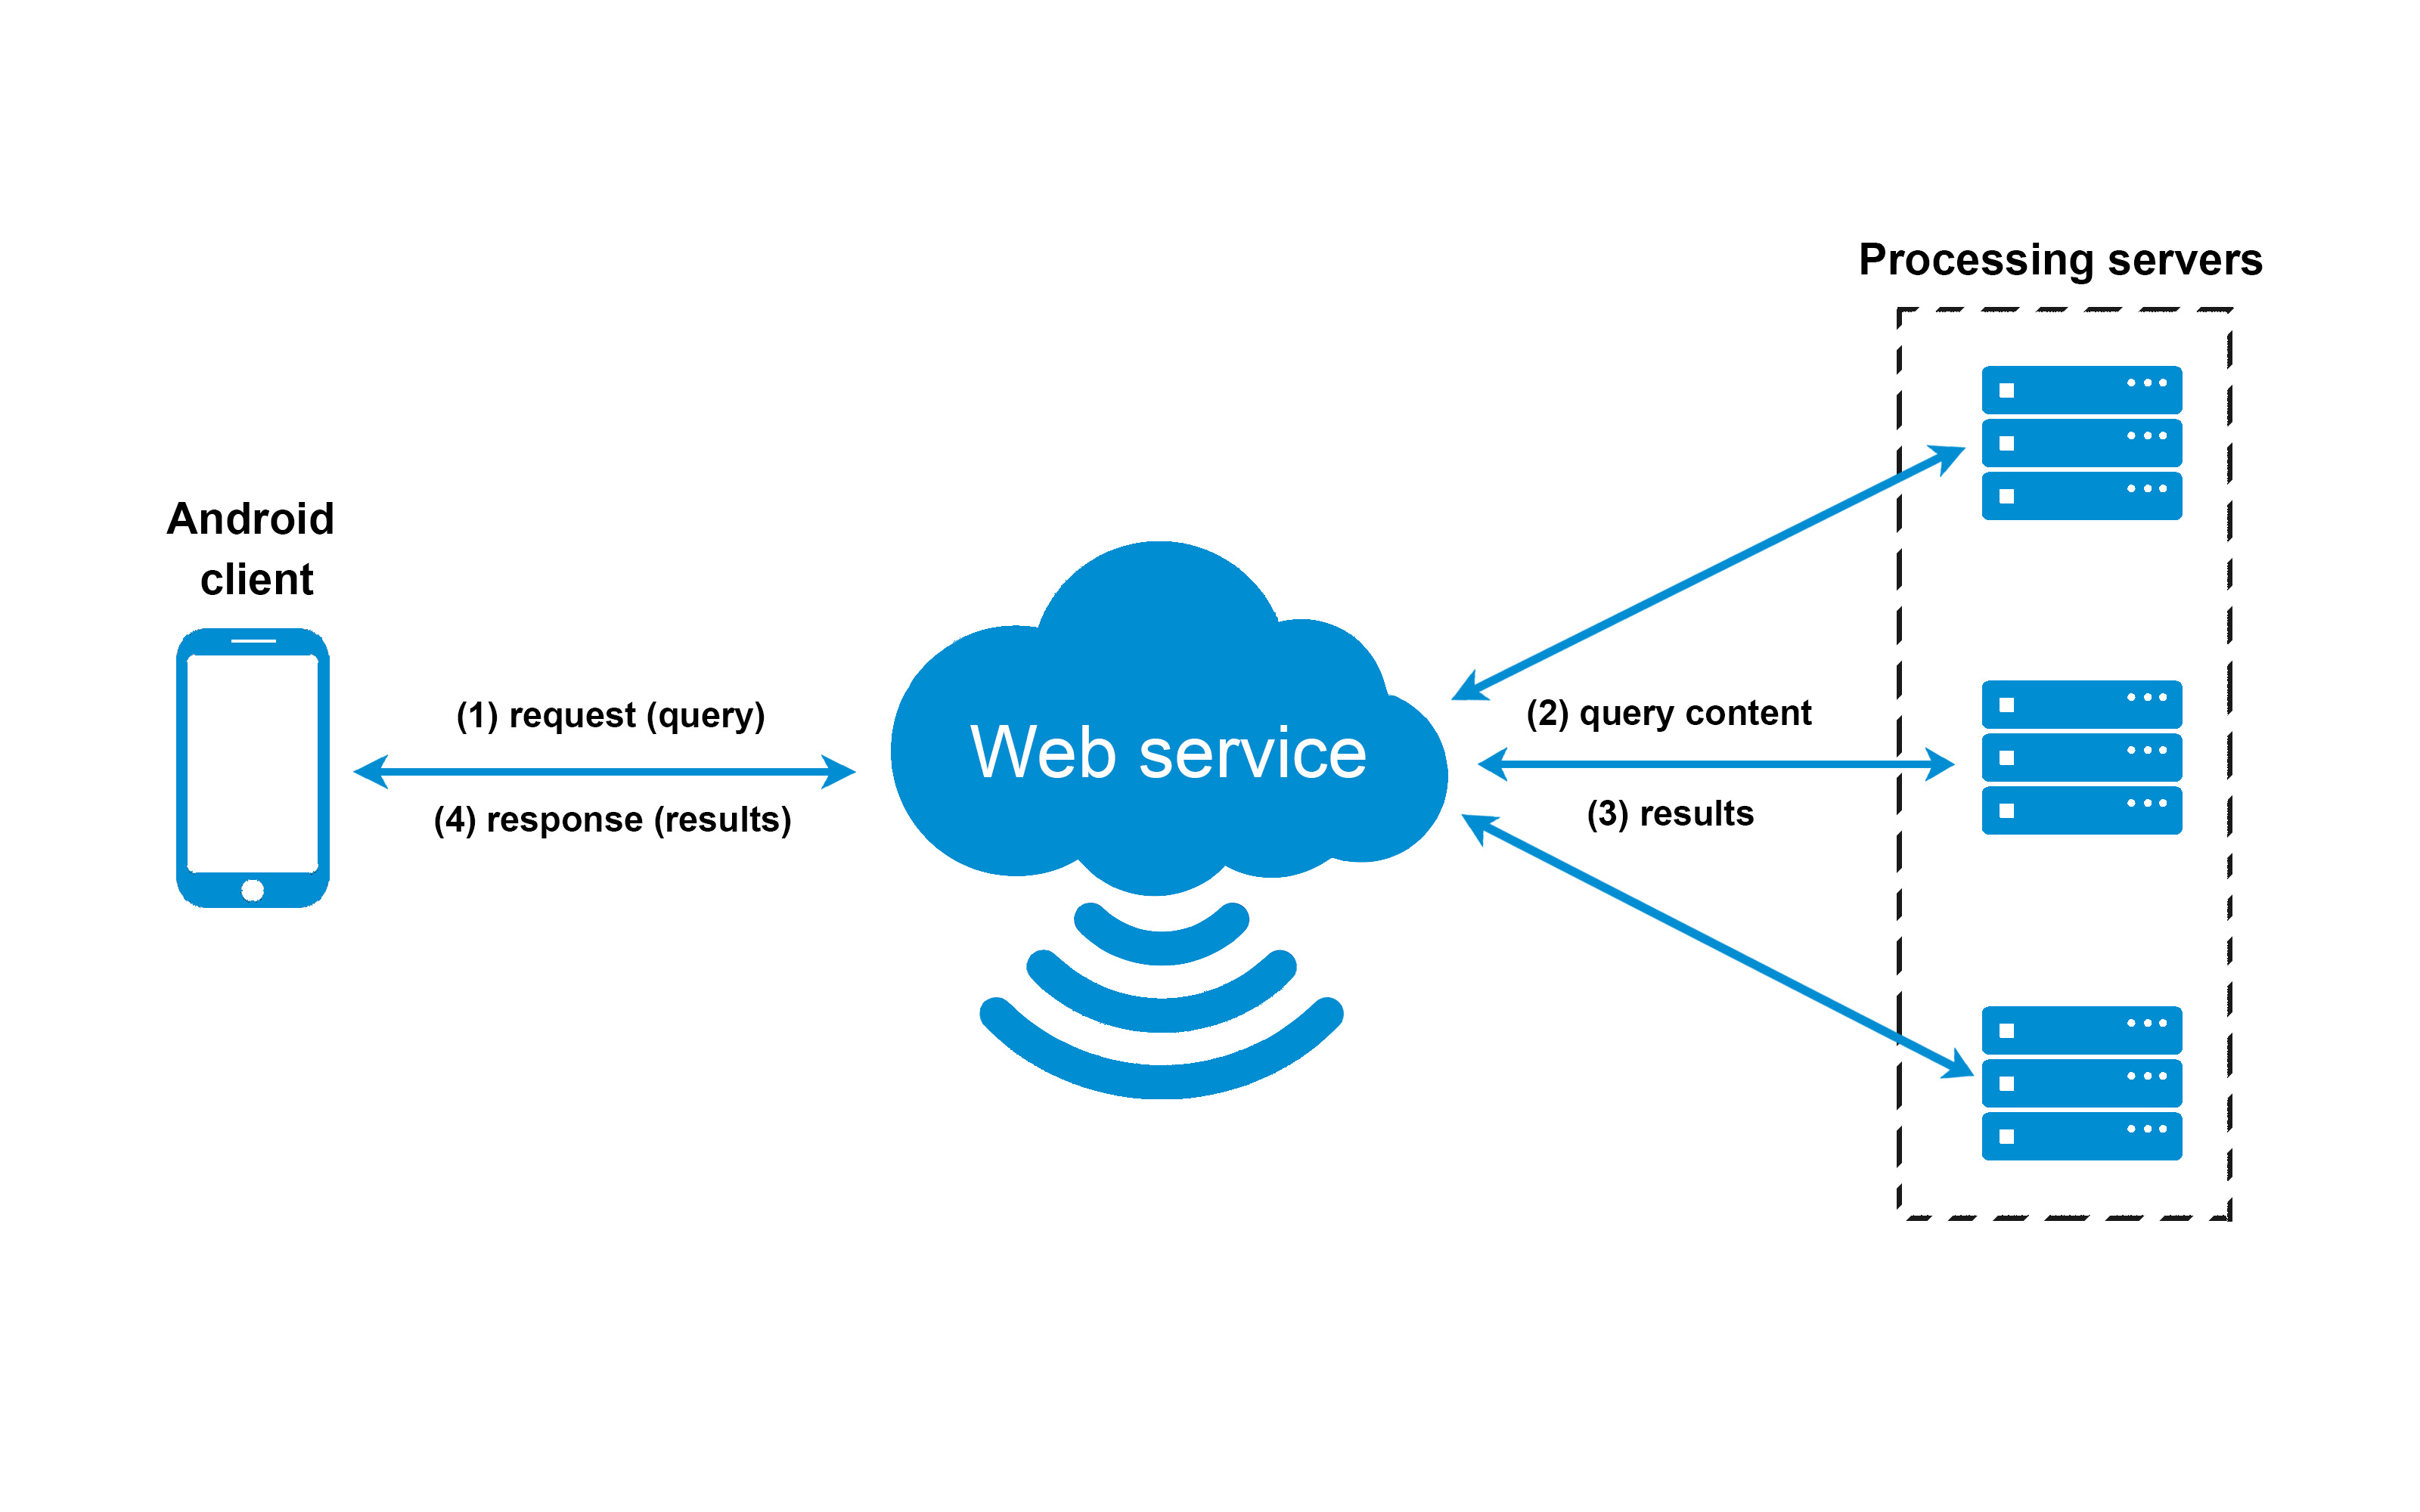
\includegraphics[scale=0.14]{architecture}
    \else
      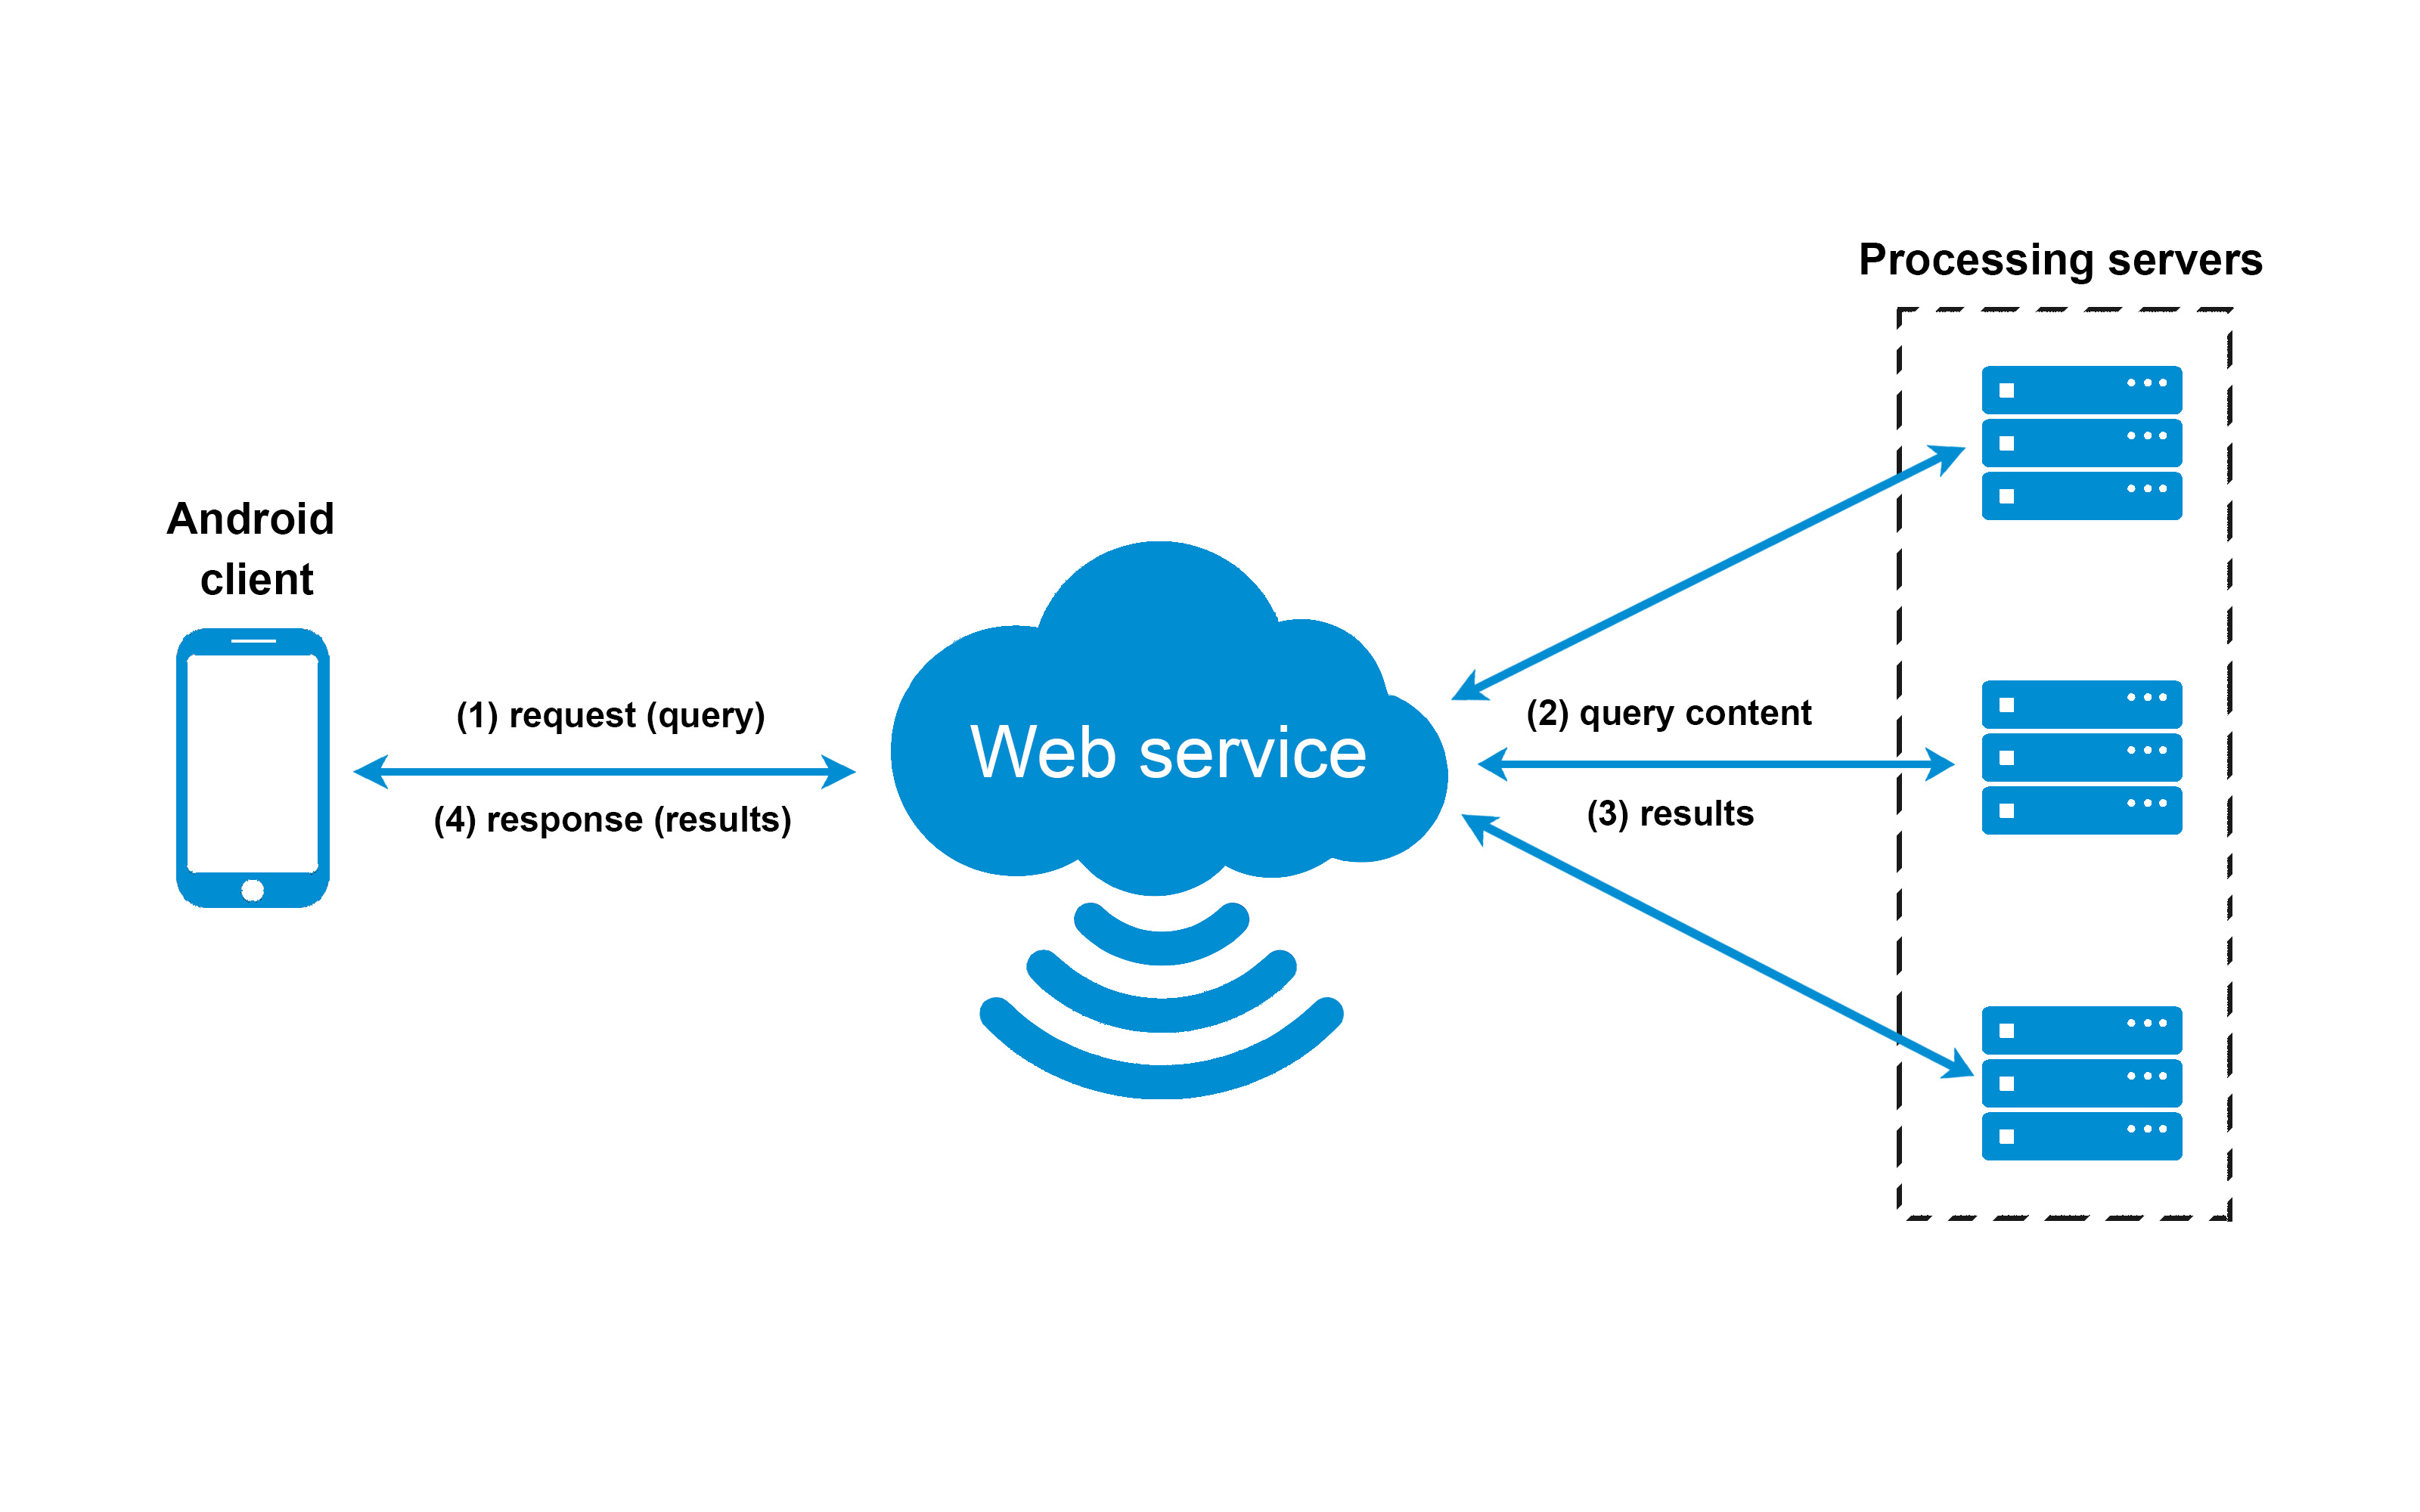
\includegraphics[scale=0.14]{architecture}
    \fi
    \caption[Kiến trúc tổng quan của hệ thống]{Kiến trúc tổng quan của hệ thống.}
    \label{FigArchitecture}
  \end{center}
\end{figure}

\subsubsection{Server side}
Server side chính là thành phần quan trọng nhất của hệ thống, thực hiện các tác vụ xử lý truy vấn. Cấu trúc của server side gồm hai thành phần chính tương ứng với hai quá trình xử lý là quá trình training và quá trình truy vấn.

-- Quá trình training: là quá trình biểu diễn lại tập dữ liệu hình ảnh, sử dụng các mô hình biểu diễn hình ảnh kết hợp với các phương pháp, kỹ thuật khác với mục đích tạo ra các dữ liệu cần thiết phục vụ quá trình truy vấn.
-- Quá trình truy vấn: là quá trình tương tác trực tiếp với hệ thống tìm kiếm đối tượng trên ảnh, nhận đầu vào là một hình ảnh, thực hiện các bước xử lý truy vấn ảnh và trả về kết quả là một tập các hình ảnh được sắp xếp theo thứ tự gần giống với hình ảnh truy vấn nhất.

\subsubsubsection{Quá trình training}
Như đã trình bày sơ lược trong mục trong mục \ref{sec:inverted-index} và \ref{experimental-setting}, quá trình training bao gồm các bước sau:

\textbf{Dò tìm, phát hiện và rút trích đặc trưng.} Từ kho dữ liệu hình ảnh được lưu sẵn trên server, bước đầu tiên của quá trình xử lý là sử dụng phương pháp phát hiện keypoint Hessian-Affine để xác định được vị trí các điểm keypoint trên hình ảnh. Từ thông tin đó, bộ SIFT descriptor mô tả và rút trích được 1 vector 128 chiều tương ứng với mỗi điểm keypoint. Những vector này sẽ được tính toán lại bằng phương pháp RootSIFT [***]. Các vector thu được chính là các tập đặc trưng của hình ảnh. 

\textbf{Gom cụm đặc trưng và xây dựng từ điển.} Các vector đặc trưng sẽ được gom cụm bằng thuật toán AKM để thu được các visual word với số lượng cụm là k = 1 triệu. Kết quả ta sẽ thu được các visual word là các từ dùng để mô tả hình ảnh. Từ những visual word này, ta sẽ xây dựng thành một từ điển để phục vụ cho việc biểu diễn hình ảnh khi truy vấn.

\textbf{Xây dựng chỉ mục ngược.} Theo như phương pháp đề xuất đã được đề cập chi tiết trong Chương \ref{chapter:proposed}, chúng tôi sẽ xây dựng chỉ mục ngược từ từ điển nhằm đạt được hiệu suất cao trong quá trình truy vấn. Cụ thể hơn, từ bộ từ điển và thông tin không gian của tất cả các visual word của mỗi hình ảnh trong bộ dữ liệu, với cấp độ phân cấp là 2, 21 chỉ mục ngược sẽ được xây dựng và lưu vào một file.

Sơ đồ xử lý cùng các thông số cài đặt được trình bày chi tiết trong phần cài đặ thí nghiệm, Hình \ref{FigInvertedFile}. Quá trình training được thực hiện độc lập trên server và là bước tiền đề cho quá trình truy vấn.

\subsubsubsection{Quá trình truy vấn}
Đây là quá trình tương tác trực tiếp với hệ thống tìm kiếm và chạy song song web service, nhận yêu cầu từ web service chuyển tiếp tới sau đó tiến hành truy vấn trả kết quả ngược trở lại web service.

Ngày nay, chất lượng hình ảnh ngày càng được tăng cao, kéo theo dung lượng hình ảnh cũng rất lớn. Việc trả về cho client một lượng lớn hình ảnh chất lượng cao là không thể vì lưu lượng và tốc độ băng thông còn bị giới hạn rất nhiều. Vì vậy sau khi xử lý truy vấn, server sẽ trả về cho client một danh sách hình ảnh thu nhỏ để đảm bảo tốc độ phản hồi. Chi tiết sẽ được trình bày rõ hơn trong phần Tối ưu hóa hệ thống ...

Việc trả về cho client các hình ảnh thu nhỏ sẽ phát sinh thêm các chức năng khác như: xem hình ảnh chất lượng tốt hơn, tải hình ảnh gốc về thiết bị. Vì vậy, tại phía server cung cấp hai chức năng chính tương ứng với hai loại yêu cầu từ phía client là yêu cầu truy vấn một hình ảnh và yêu cầu tải một (hoặc một tập) các hình ảnh theo các mức chất lượng khác nhau.

Với yêu cầu như trên, các server được chia làm 2 loại chính:
-- Server truy vấn: tiếp nhận yêu cầu truy vấn hình ảnh, xử lý và trả về kết quả là danh sách xếp hạng cùng một phần các hình ảnh thu nhỏ giống với hình truy vấn nhất.
-- Server tải hình ảnh: tiếp nhận yêu cầu tải hình ảnh, trả về hình ảnh được lất từ bộ nhớ.

\begin{figure}[!htbp]
  \begin{center}
    \leavevmode
    \ifpdf
      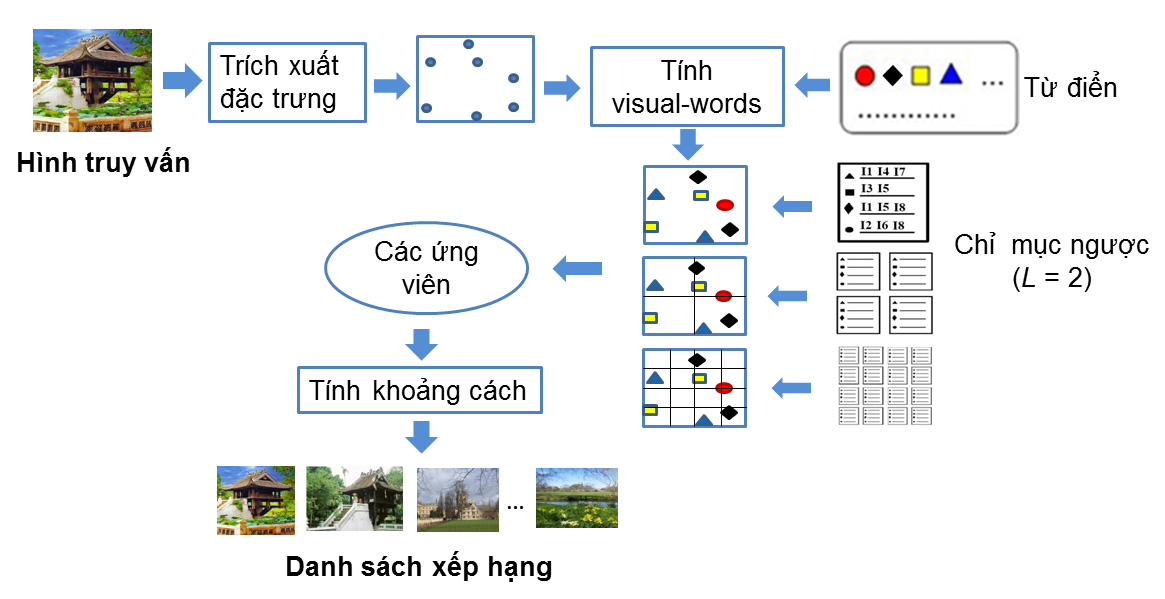
\includegraphics[scale=0.14]{query-process-server}
    \else
      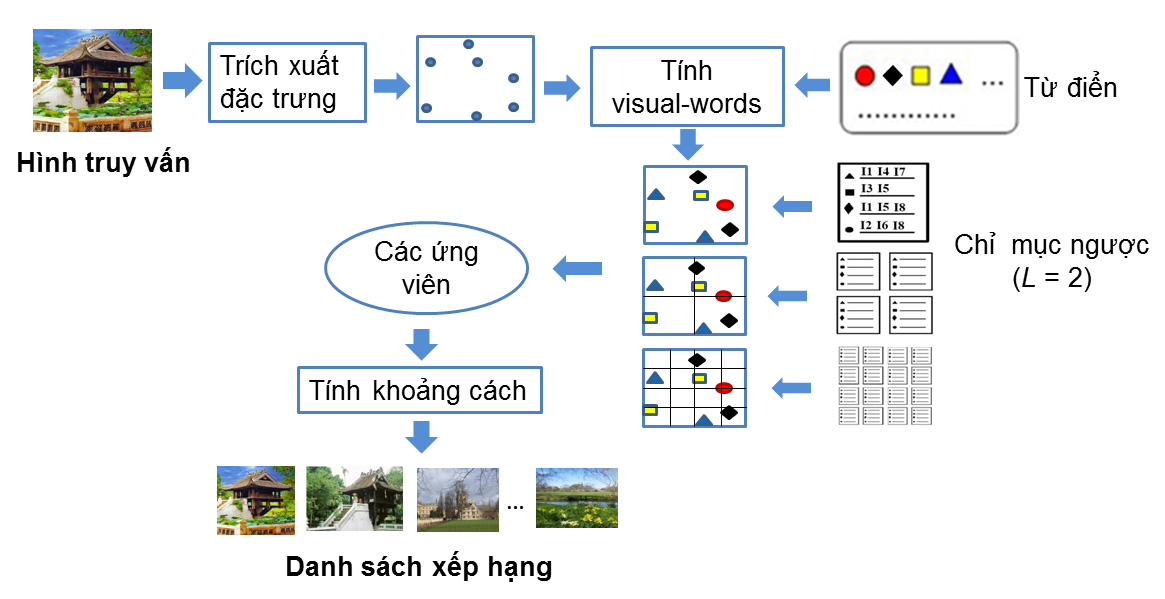
\includegraphics[scale=0.14]{query-process-server}
    \fi
    \caption[Kiến trúc tổng quan của hệ thống]{Kiến trúc tổng quan của hệ thống.}
    \label{query-process-server}
  \end{center}
\end{figure}

Quá trình xử lý truy vấn được đã trình bày chi tiết trong mục \ref{sec:intergrated} và được thể hiện trong Hình \ref{query-process-server}. Đầu tiên, ta sẽ rút trích đặc trưng từ hình ảnh truy vấn. Sau đó các đặc trưng này được đưa vào từ điển để lấy được các visual word tương ứng. Từ các visual word và vị trí của nó trên hình ảnh, ta sẽ dùng chỉ mục ngược đề xuất để tìm kiếm các hình ảnh ứng viên có liên quan và đồng thời tính khoảng cách từ hình truy vấn tới các hình ảnh này. Sau đó, danh sách hình ảnh ứng viên sẽ được sắp xếp theo mức độ tượng tự từ cao tới thấp. Kết quả sẽ được server gửi ngược trở về webservice và trả về cho client yêu cầu.

\subsubsection{Web service}
Web service là thành phần trung gian đóng vai trò phân phối các yêu cầu từ phía client tới các server xử lý. Thành phần này sử dụng dịch vụ web {cite\} chạy trên web server cung cấp các phương thức giúp client và server xử lý kết nối, truyền tải các dữ liệu cần thiết.

Với một hệ thống tìm kiếm cơ bản sử dụng từ khóa thông thường, thành phần xử lý có thể chính là web service. Với mỗi yêu cầu tìm kiếm, nó sẽ tạo ra một tiến trình và truy xuất tới cơ sở dữ liệu để lấy thông tin một cách nhanh chóng, có thể đáp ứng nhiều yêu cầu đồng thời, phụ thuộc vào phần cứng và các thiết lập trên nó. Nhưng với một hệ thống tìm kiếm hình ảnh, chi phí tính toán và tài nguyên phục vụ quá trình tìm kiếm rất lớn, việc tạo ra nhiều tiến trình xử lý là không khả thi. Nếu giới hạn số lượng yêu cầu ở mức thấp để đảm bảo an toàn cho hệ thống thì sẽ không đáp ứng được yêu cầu thực tế, ngược lại nếu không kiểm soát các yêu cầu truy vấn thì hệ thống có thể sẽ không đáp ứng được và dễ dàng bị quá tải dẫn dến nguy hiểm cả cho phần cứng. Chính vì vậy, giải pháp tốt nhất chính là chia tải, bằng cách sử dụng nhiều server xử lý và chuyển tiếp các yêu cầu truy vấn tới các server này. Từ đó có thể xử dụng hai cách kết nối:
-- Cách 1: Web service lưu giữ thông tin các server xử lý, và khi có yêu cầu từ phía client, nó sẽ gửi thông tin của server để client trực tiếp kết nối và truyền tải dữ liệu tới server xử lý.
-- Cách 3: Web service nhận yêu cầu từ phía client, truyền tải dữ liệu tới server xử lý, chờ kết quả xử lý từ server và gửi lại cho client. Như vậy client không được phép kết nối trực tiếp tới server xử lý.

Để giải quyết vấn đề trên, 

 Do đó, web service thực hiện hai nhiệm vụ chính là nhận các request từ các client gửi lên, điều phối để cân bằng tải giữa các server và nhận kết quả trả về từ server để trả lại đúng cho client tương ứng.

Trước tiên, các request do client gửi lên sẽ được đưa vào hàng đợi. Các kết nối của phía server gửi lên cũng được đưa vào một hàng đợi. Controller sẽ làm nhiệm vụ kiểm tra xem liệu có kết nối của server nào đang đợi không để chuyển tiếp request của client đến server đó. Đồng thời, bằng việc sử dụng kỹ thuật long polling, request của client sẽ không được trả về ngay mà sẽ bị giữ lại để chờ đợi kết quả từ phía server. Sau khi xử lý và lấy được kết quả, server sẽ gửi lại kết quả cho controller và controller sẽ phản hồi request của client đang chờ.

Sơ đồ mô hình hoạt động chi tiết của web service được thể hiện trong Hình \ref{FigWS}.

\begin{figure}[!htbp]
  \begin{center}
    \leavevmode
    \ifpdf
      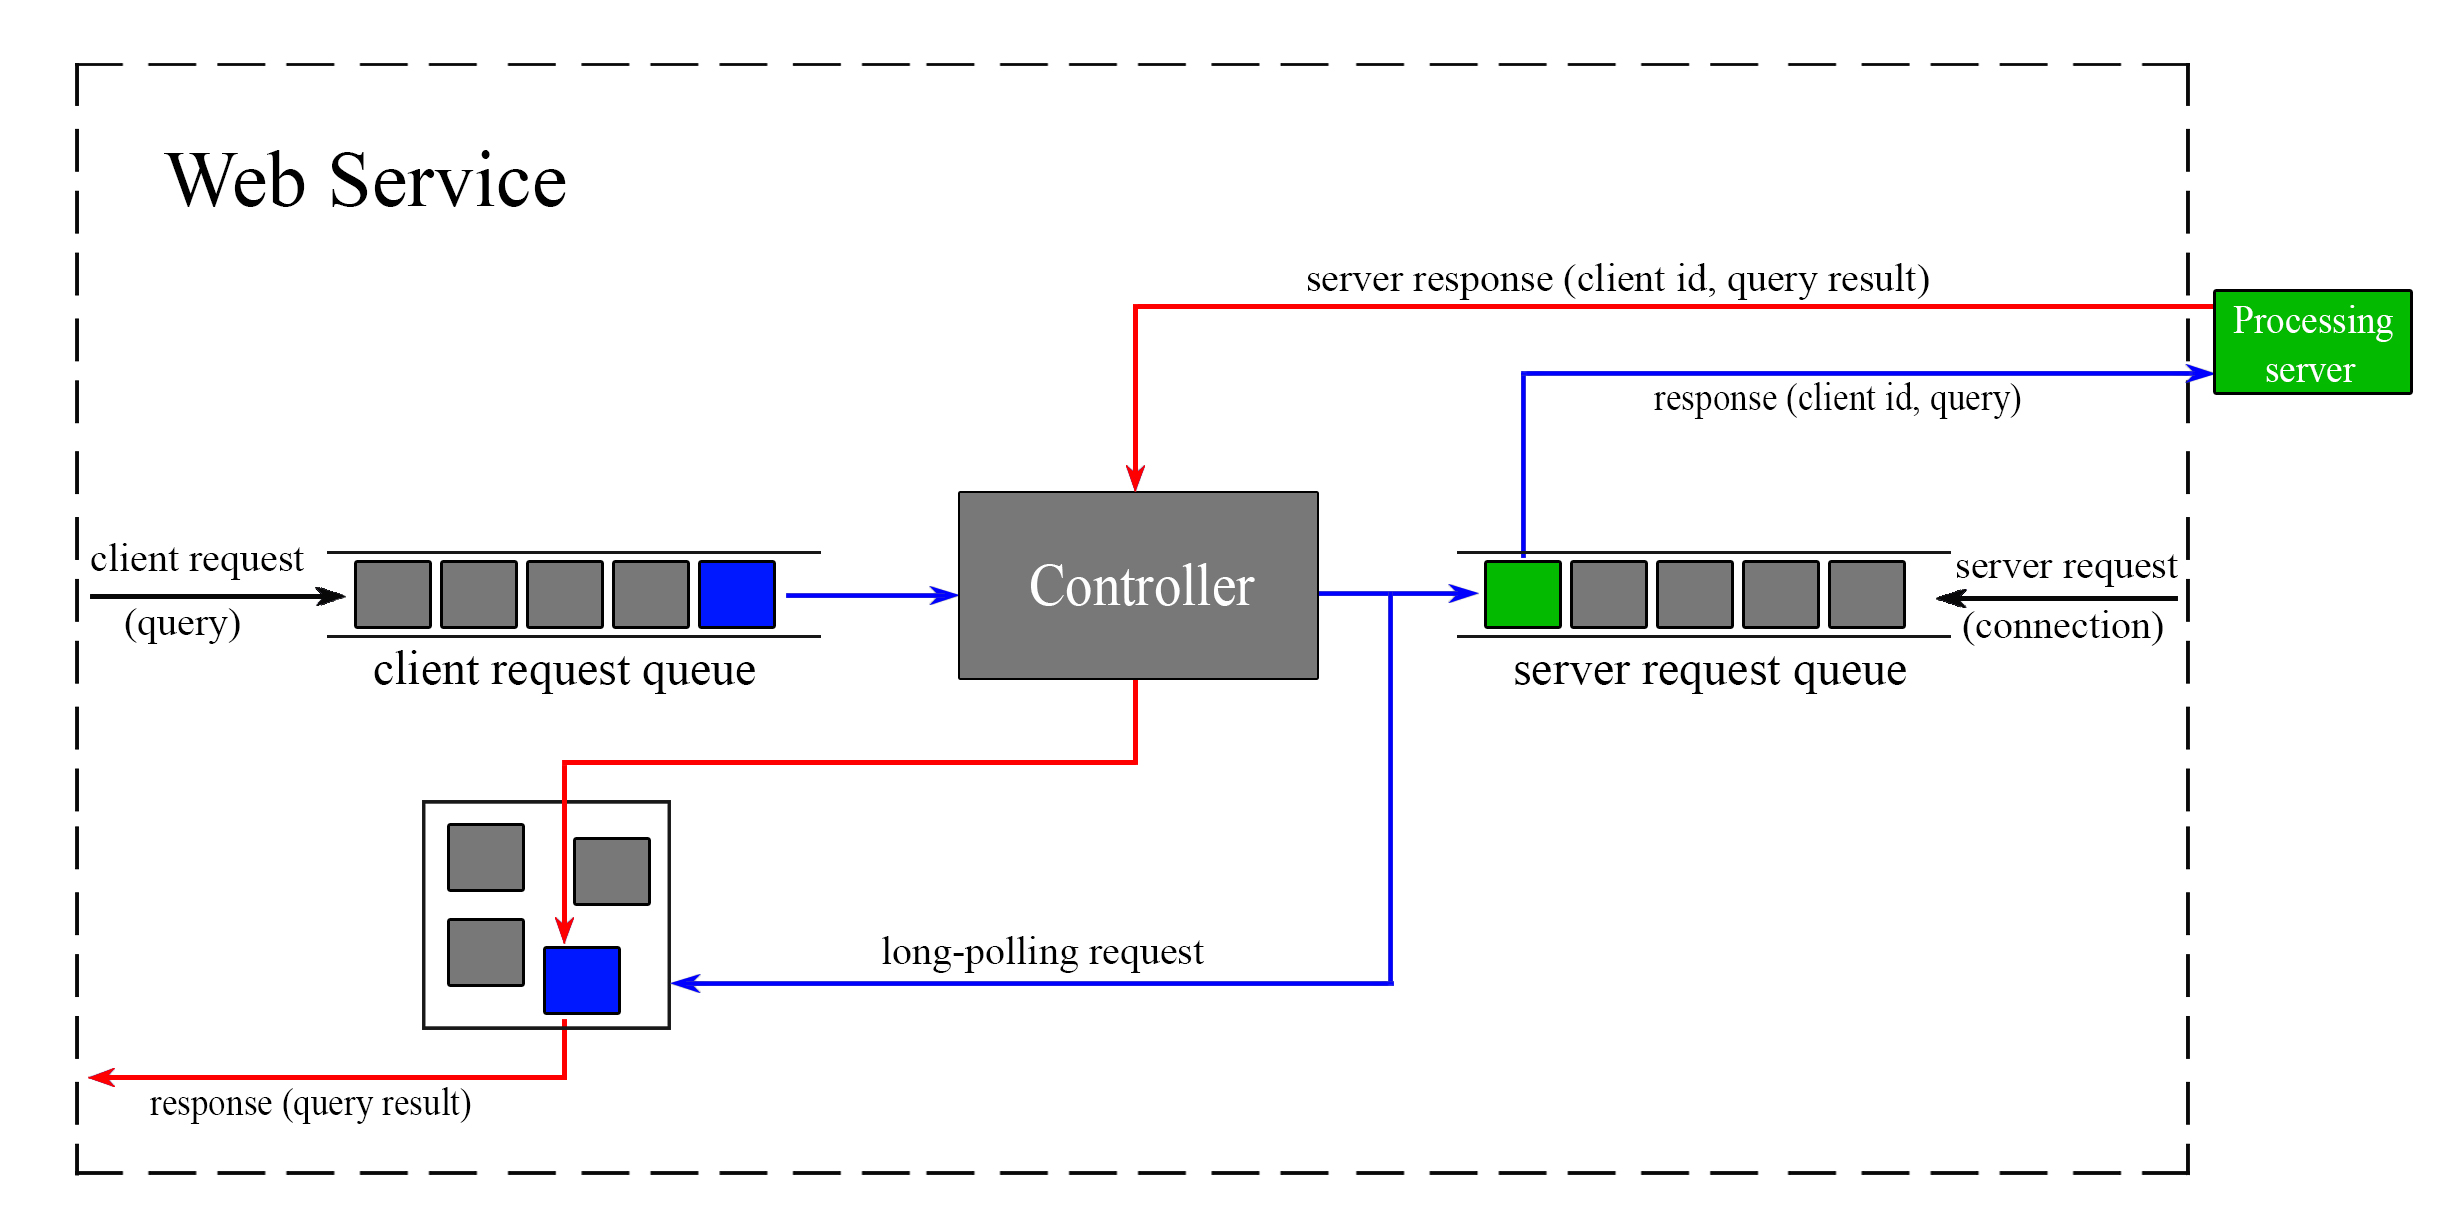
\includegraphics[scale=0.17]{ws_model}
    \else
      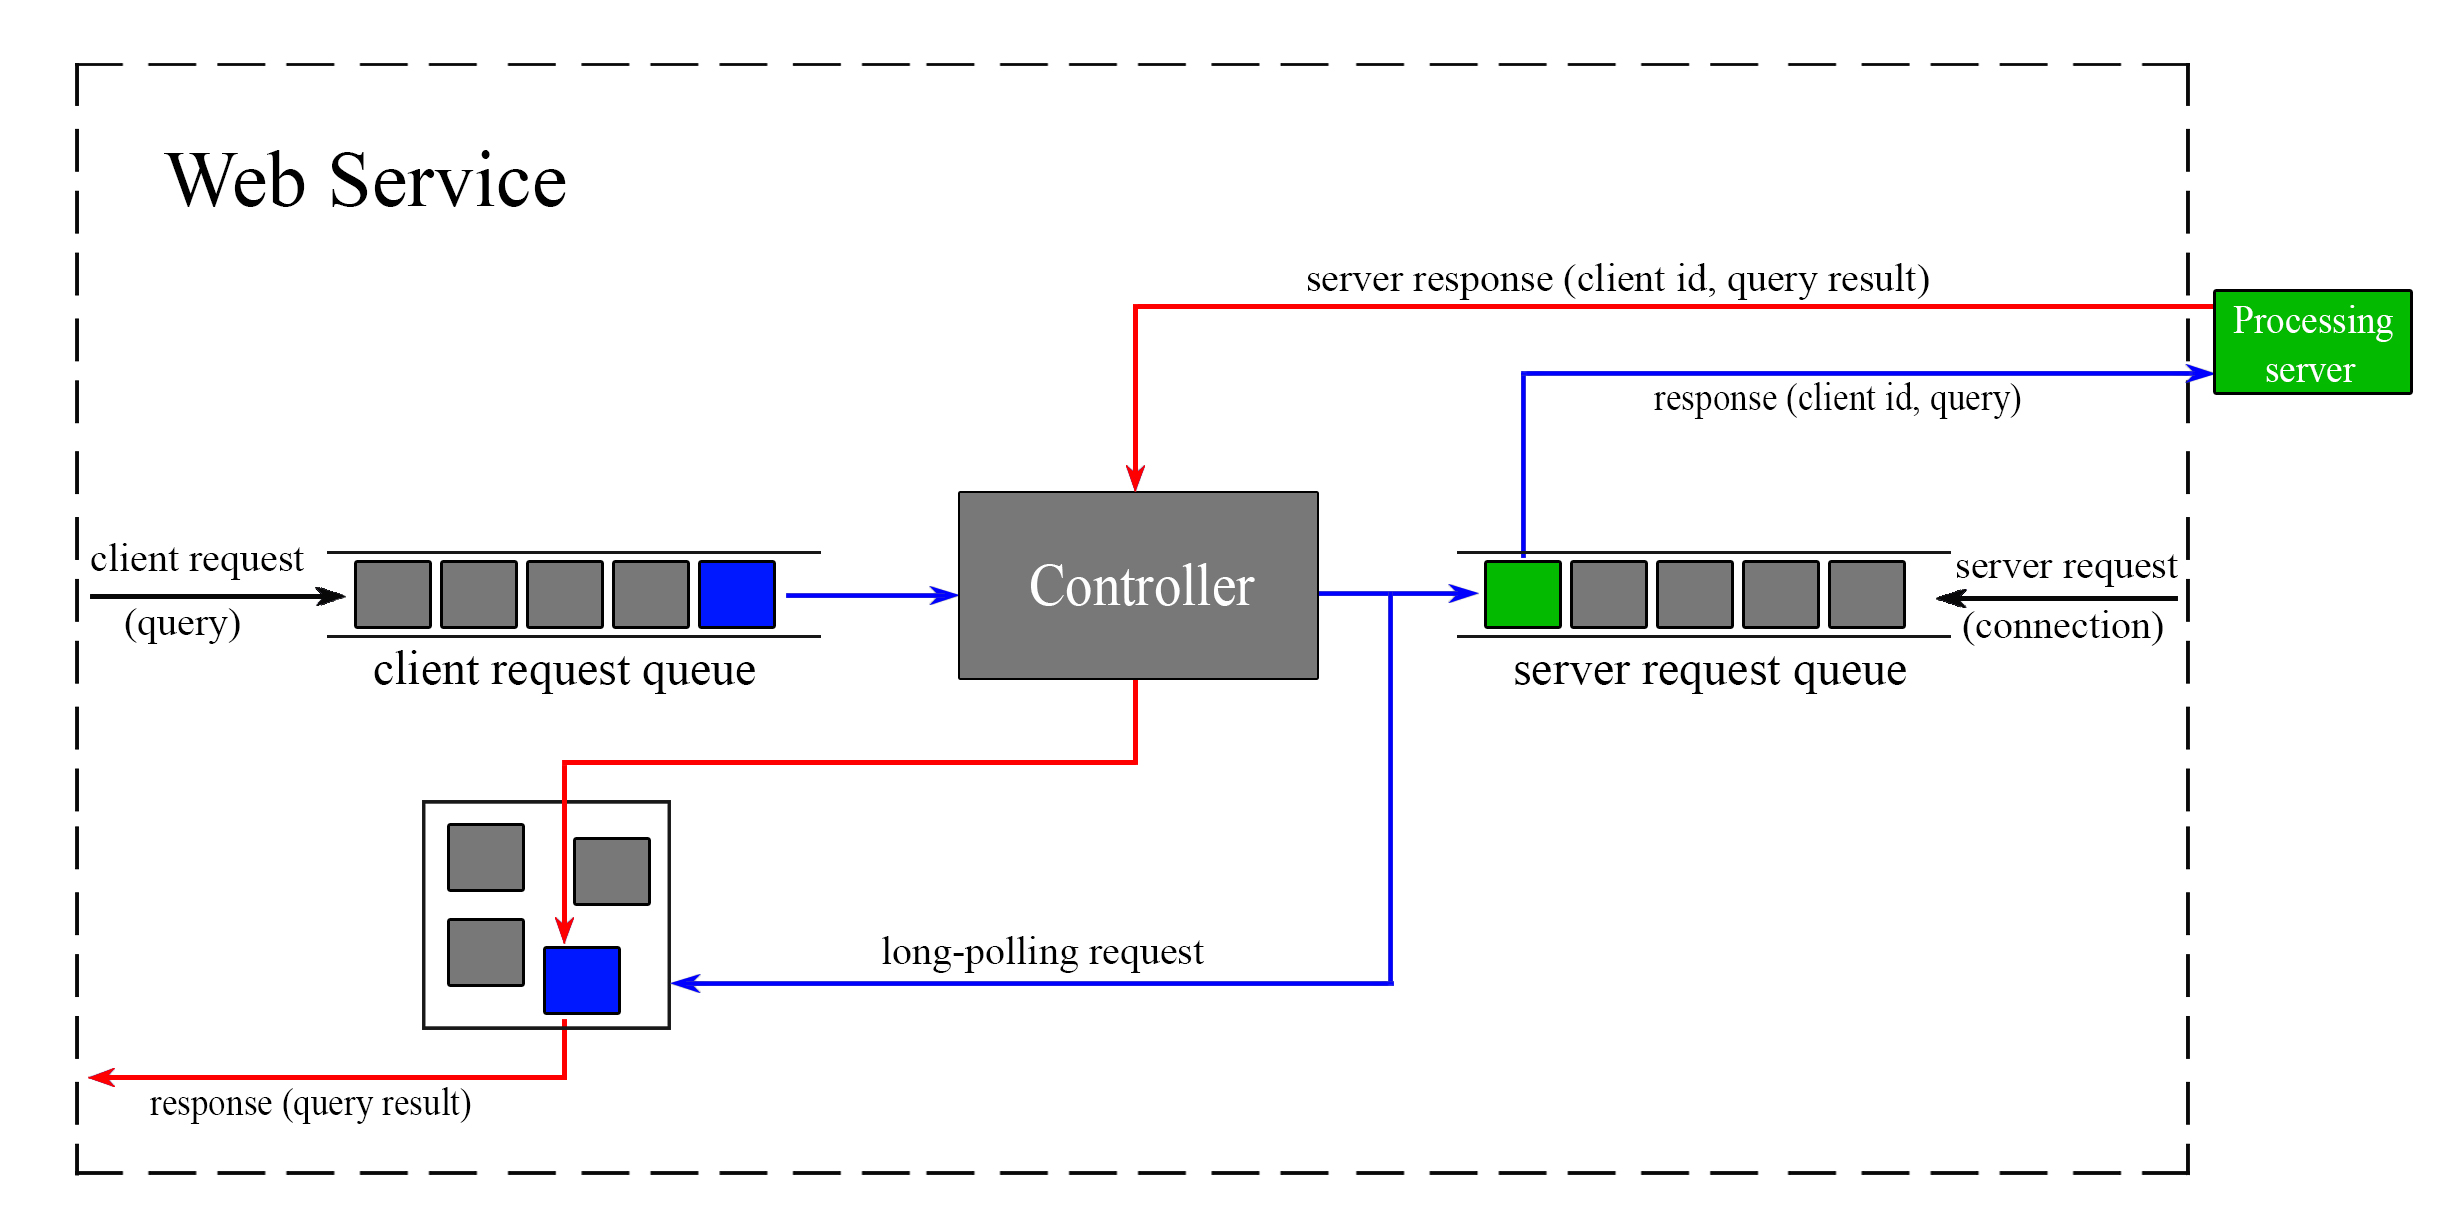
\includegraphics[scale=0.17]{ws_model}
    \fi
    \caption[Sơ đồ mô hình hoạt động chi tiết của web service]{Sơ đồ mô hình hoạt động chi tiết của web service.}
    \label{FigWS}
  \end{center}
\end{figure}


\subsubsection{Client side}
Nhiệm vụ của client là cung cấp cho người dùng một giao diện để tương tác trong quá trình chọn ảnh để request. Do đó nó cần đáp ứng được các yêu cầu về giao diện thân thiện, tiện dụng và cung cấp đầy đủ các chức năng cho người dùng. Hình \ref{FigAndroidClient} cho thấy kiến trúc tổng quan của client side.

\begin{figure}[!htbp]
  \begin{center}
    \leavevmode
    \ifpdf
      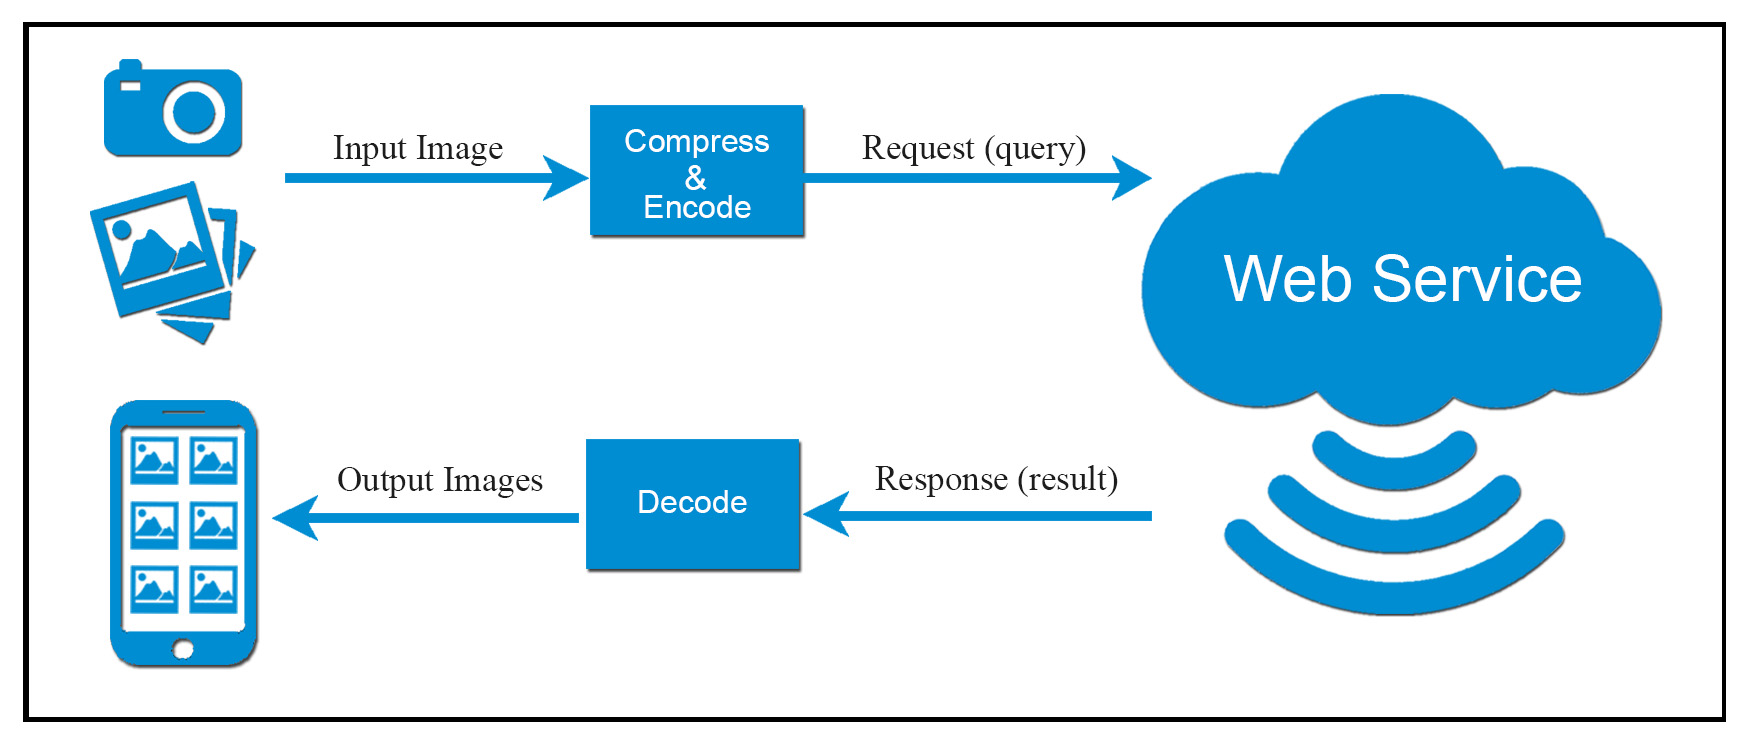
\includegraphics[scale=0.25]{android_client}
    \else
      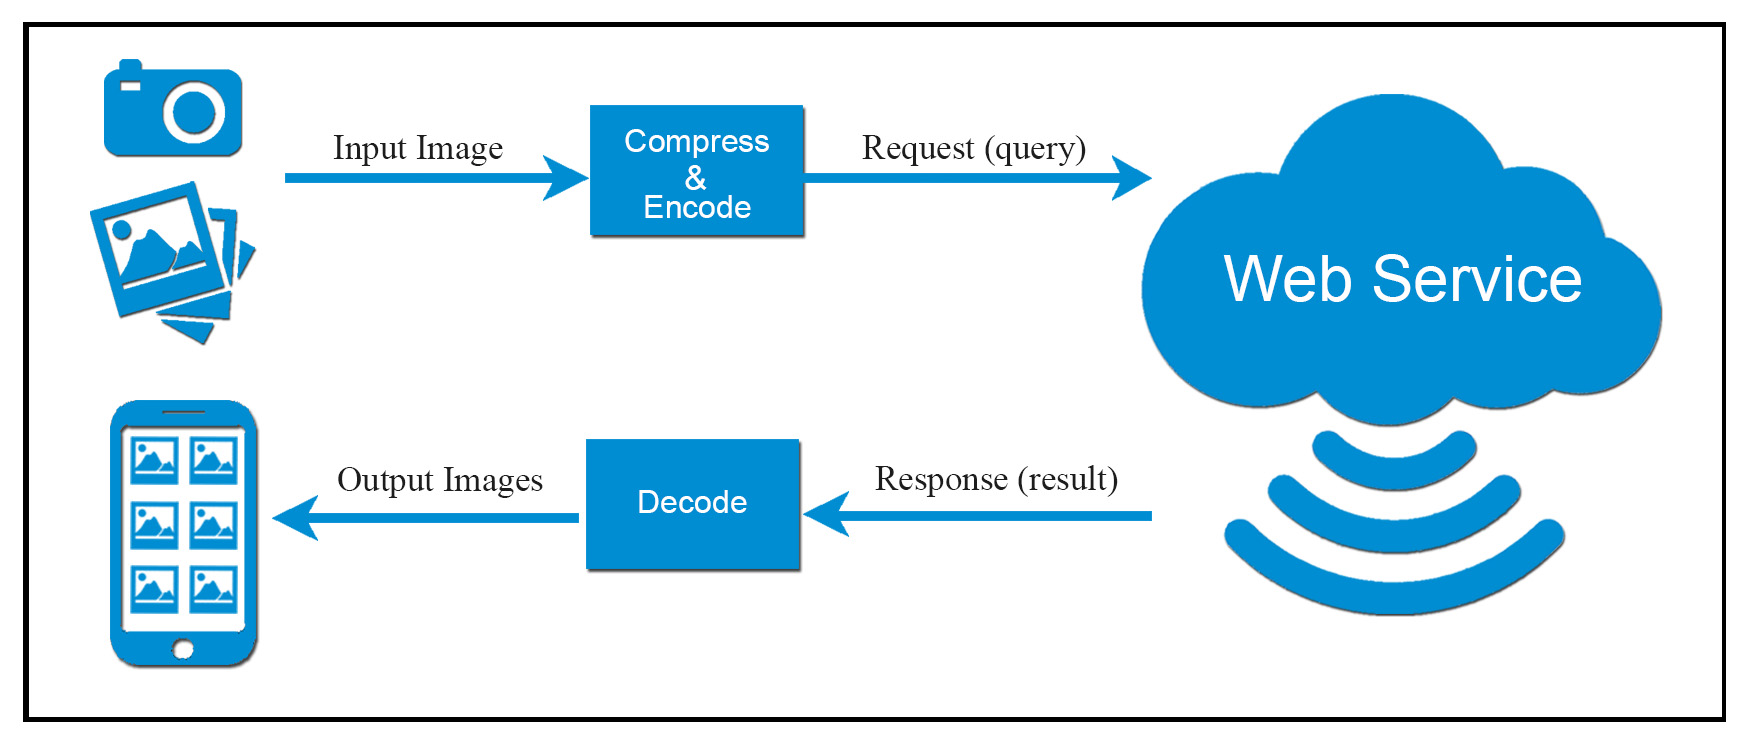
\includegraphics[scale=0.25]{android_client}
    \fi
    \caption[Kiến trúc của client side]{Kiến trúc của client side.}
    \label{FigAndroidClient}
  \end{center}
\end{figure}

Ứng dụng client được xây dựng đơn giản và thân thiện với người dùng. Nó cho phép người dùng được chọn hình ảnh từ camera hoặc hình ảnh được lưu trữ trong bộ nhớ. Để nâng cao độ chính xác, người dùng có thể dùng tay để quét chọn vùng hình ảnh có chứa đối tượng mà mình muốn truy vấn. Sau đó hình ảnh sẽ được gửi cho web service. Và khi có kết quả trả về từ web service, ứng dụng sẽ hiển thị danh sách các hình ảnh trả về dưới dạng các thumbnail. Nếu người dùng muốn xem hình ảnh lớn hơn, chỉ cần chọn hình ảnh và ứng dụng sẽ gửi request lên web service để lấy hình ảnh chất lượng cao về và hiển thị.

Chi tiết tổ chức của các lớp được thể hiện trong Hình \ref{FigClientFramework}.

\begin{figure}[!htbp]
  \begin{center}
    \leavevmode
    \ifpdf
      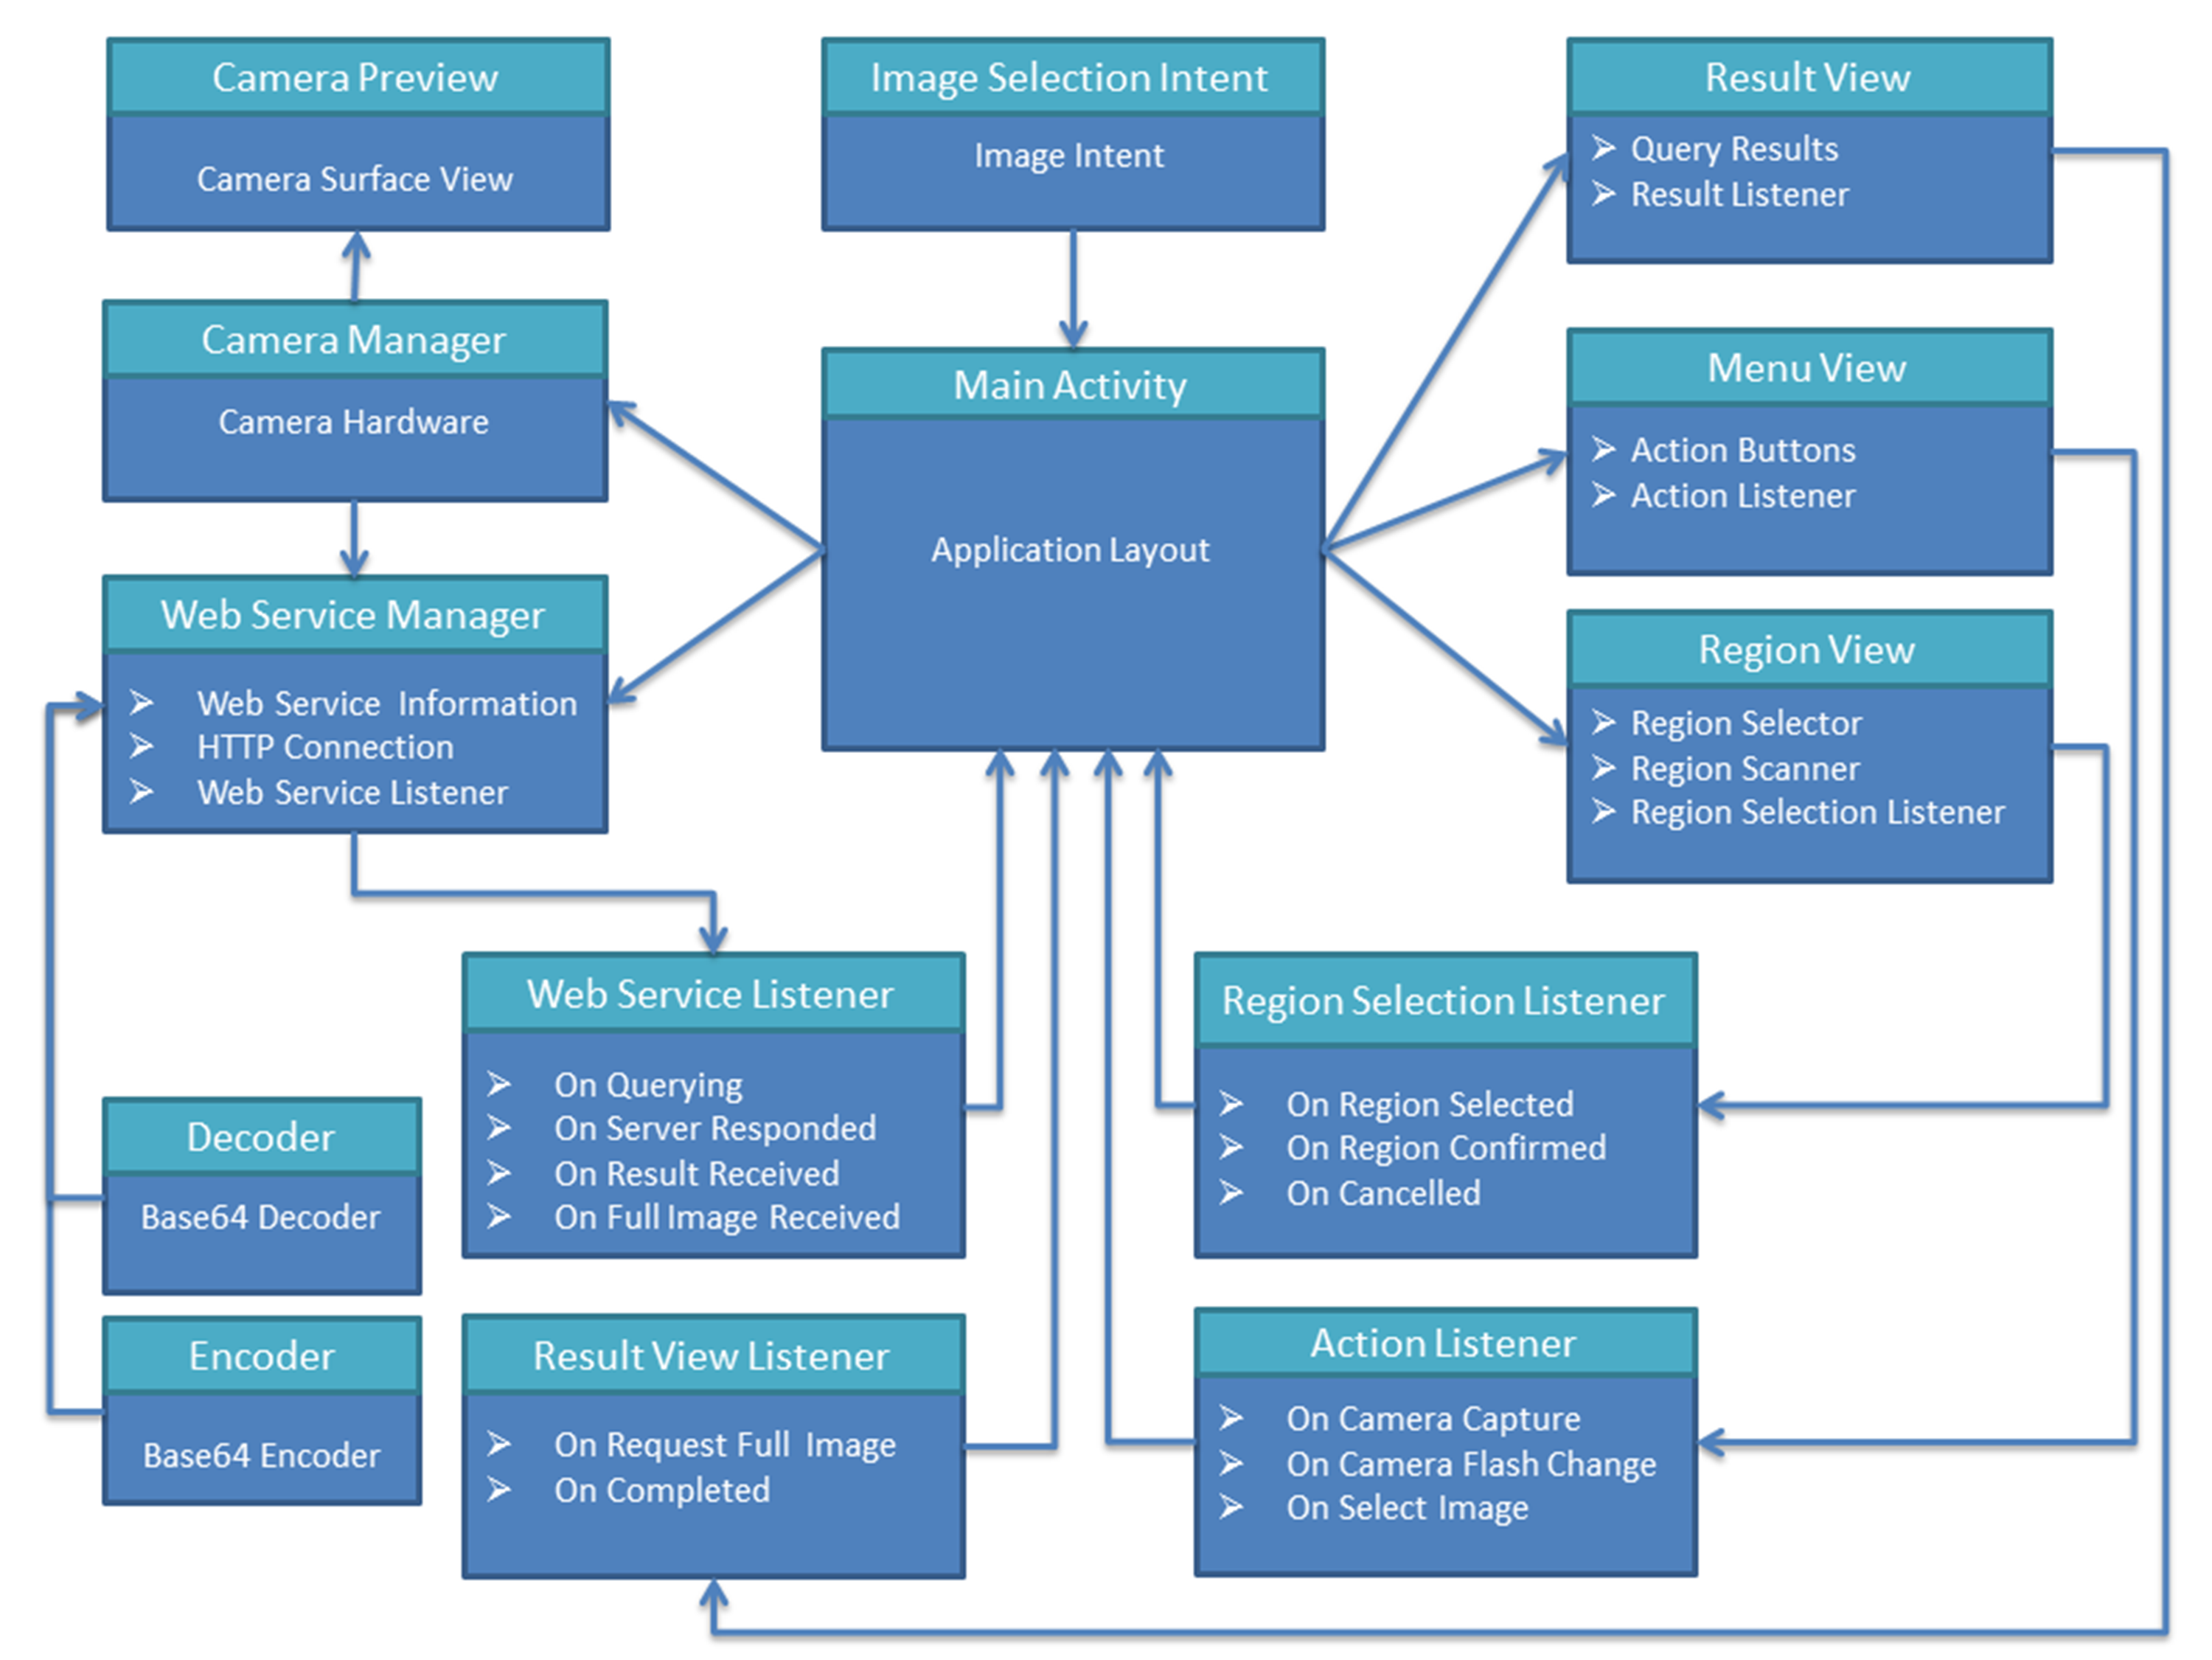
\includegraphics[scale=0.19]{client_framework}
    \else
      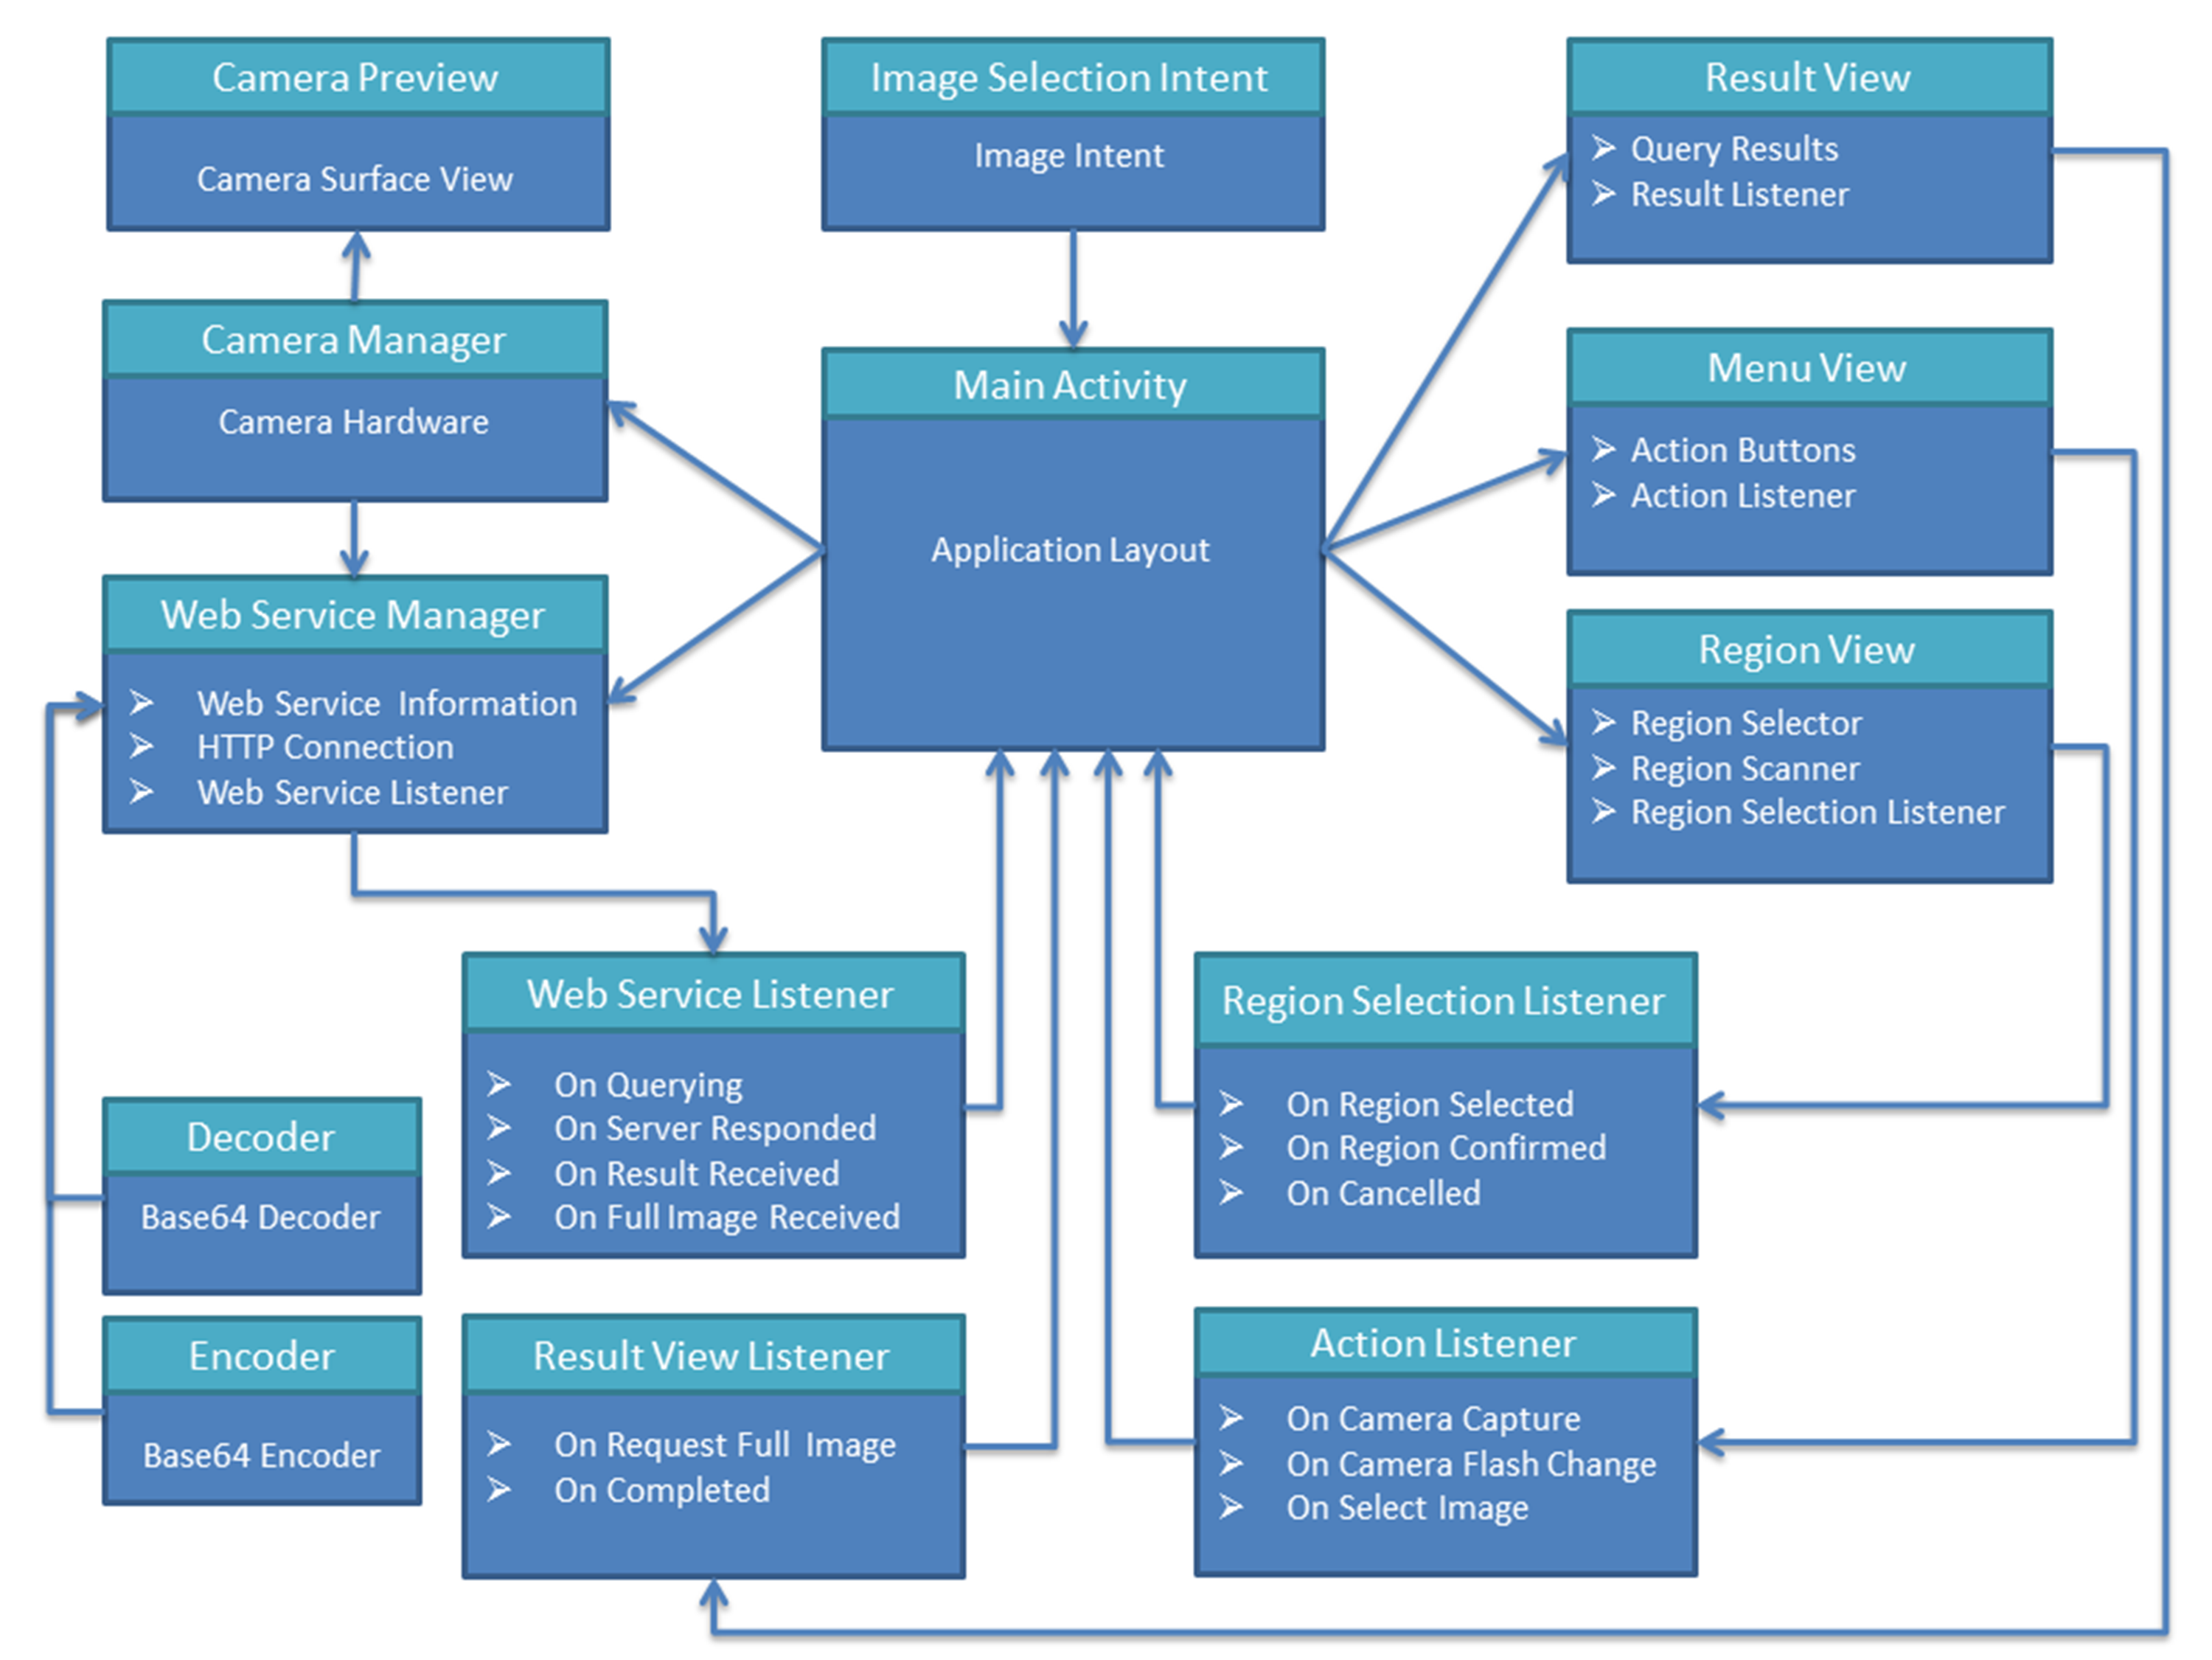
\includegraphics[scale=0.19]{client_framework}
    \fi
    \caption[Sơ đồ tổ chức các lớp của client side]{Sơ đồ tổ chức các lớp của client side.}
    \label{FigClientFramework}
  \end{center}
\end{figure}

\subsection{Giao diện}
Giao diện của ứng dụng được thiết kế đơn giản và tiện dụng với người sử dụng. Các hình ảnh screenshot của ứng dụng được thể hiện trong các hình \ref{FigChooseRegion}, \ref{FigProcessing} và \ref{FigResultCapture}.

\begin{figure}[!htbp]
  \begin{center}
    \leavevmode
    \ifpdf
      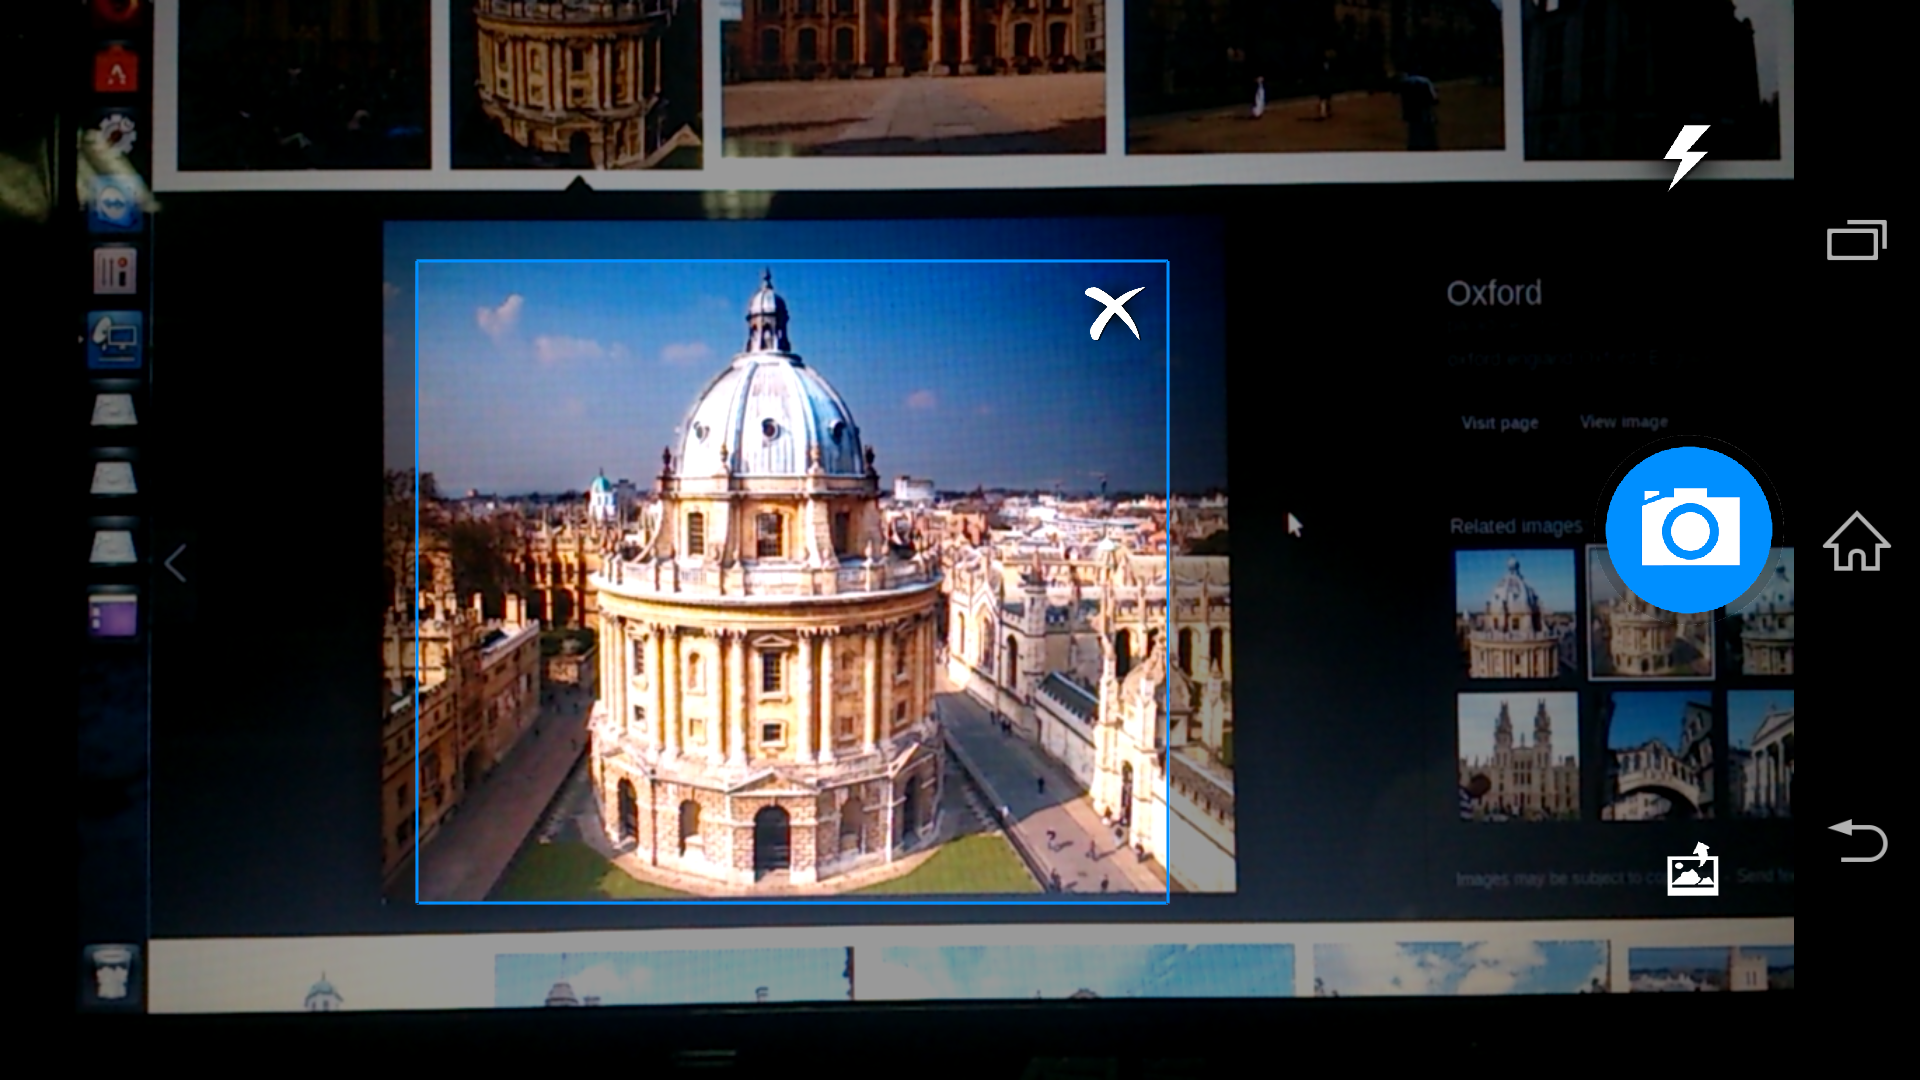
\includegraphics[scale=0.17]{choose_region}
    \else
      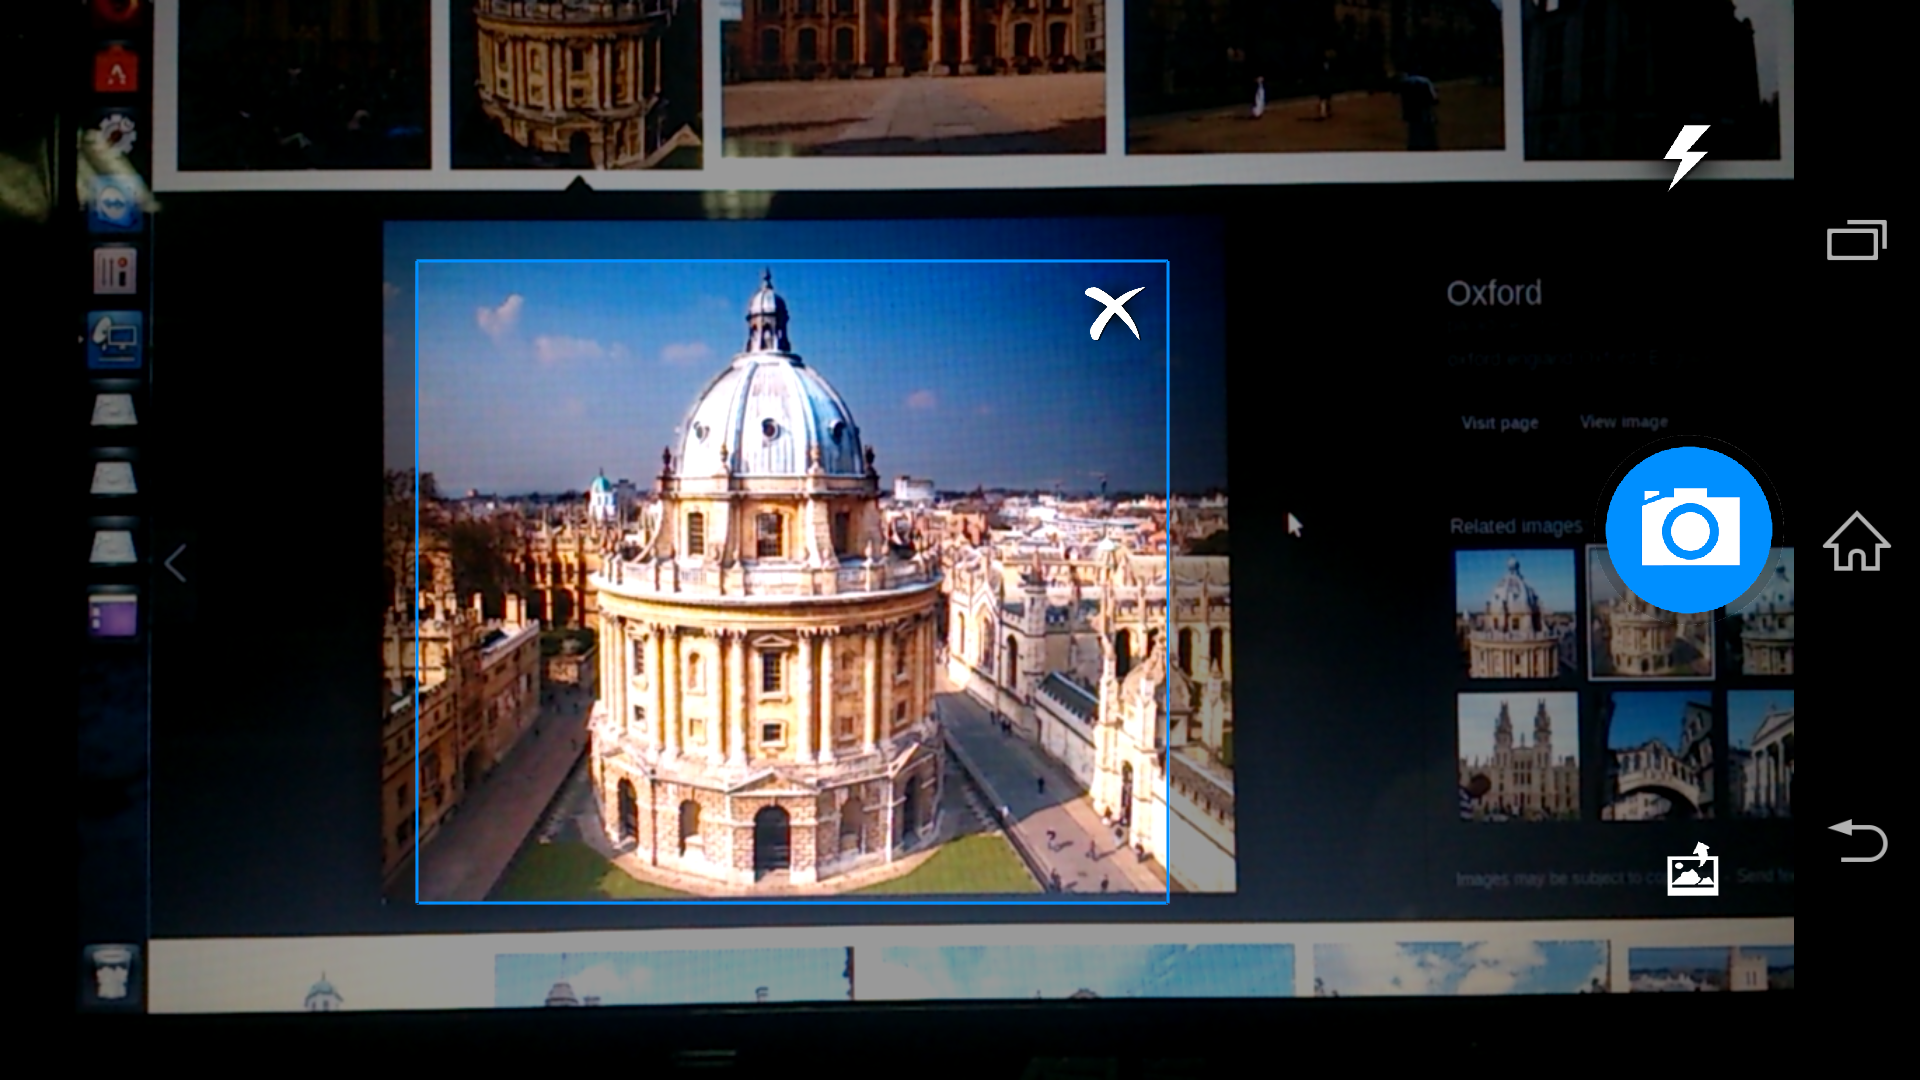
\includegraphics[scale=0.17]{choose_region}
    \fi
    \caption[Hình ảnh ứng dụng khi chọn vùng ảnh truy vấn]{Hình ảnh ứng dụng khi chọn vùng ảnh truy vấn.}
    \label{FigChooseRegion}
  \end{center}
\end{figure}

\begin{figure}[!htbp]
  \begin{center}
    \leavevmode
    \ifpdf
      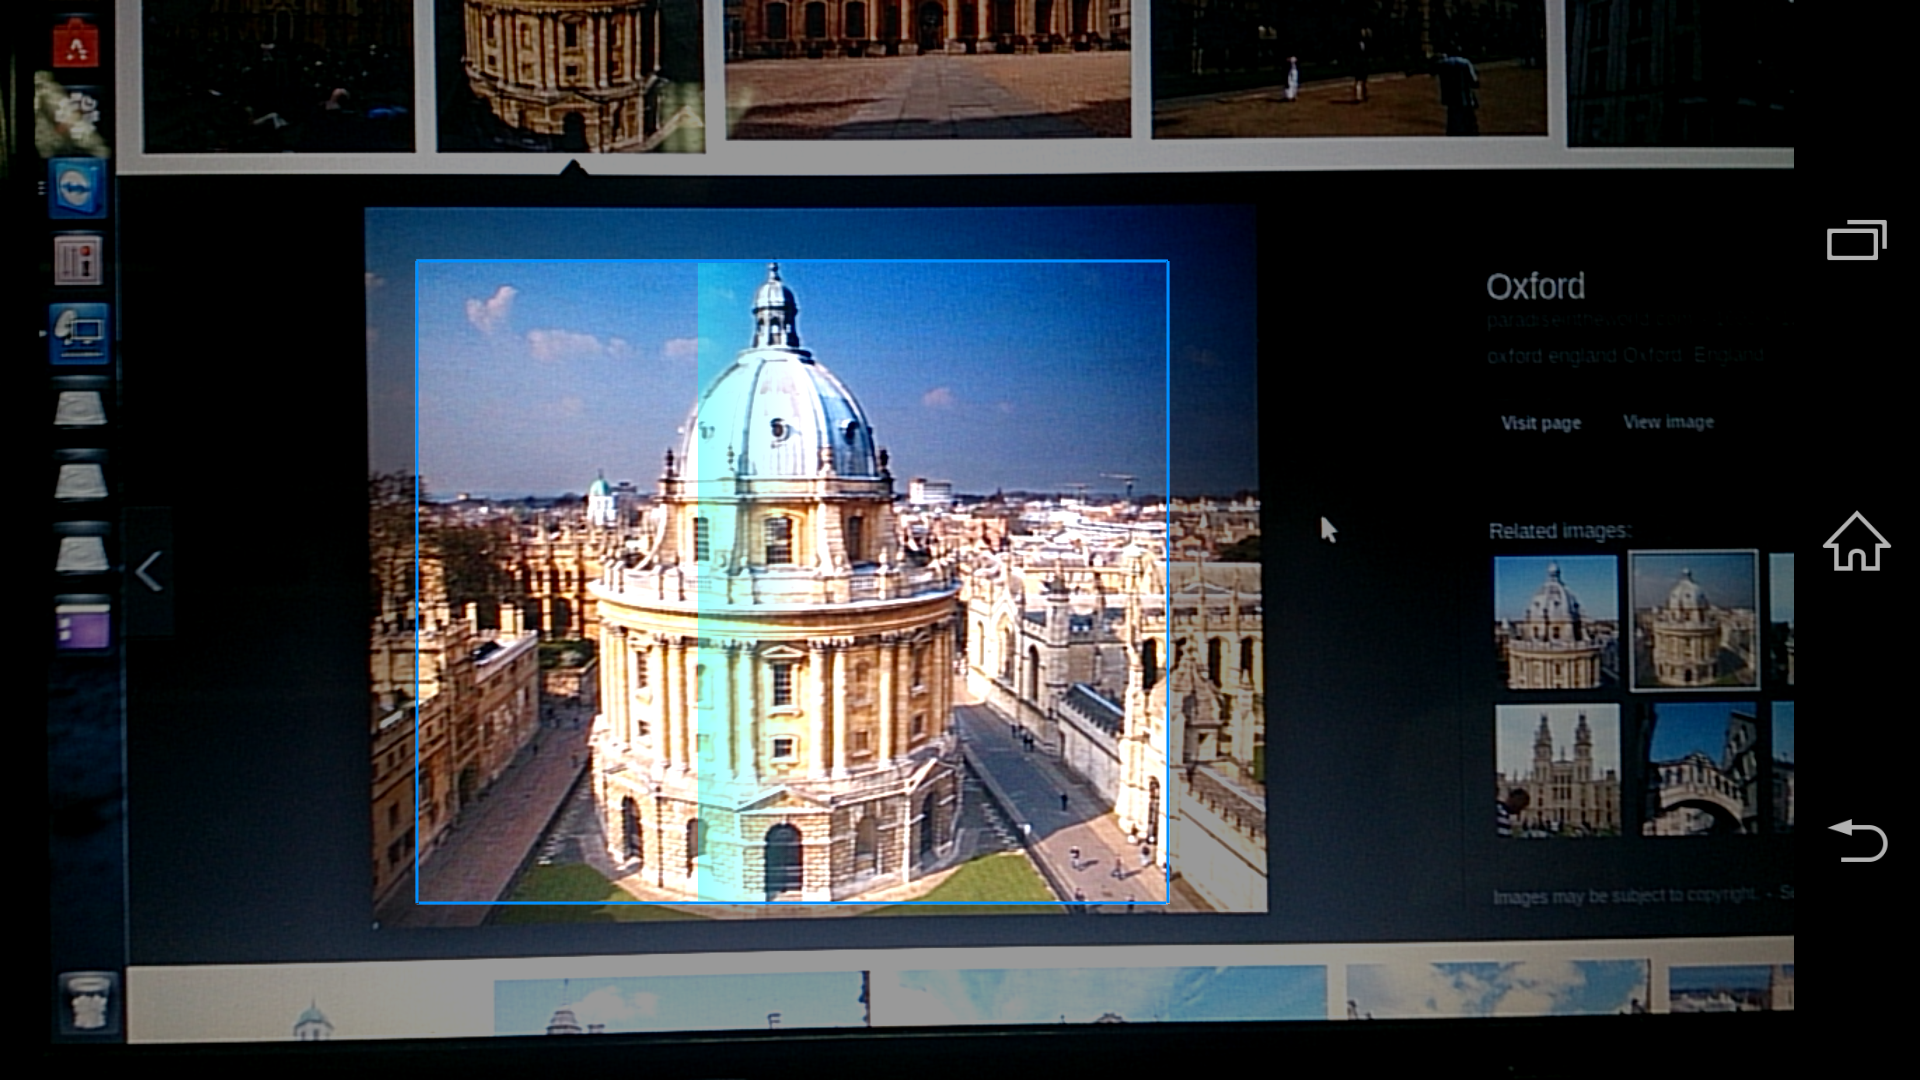
\includegraphics[scale=0.17]{processing}
    \else
      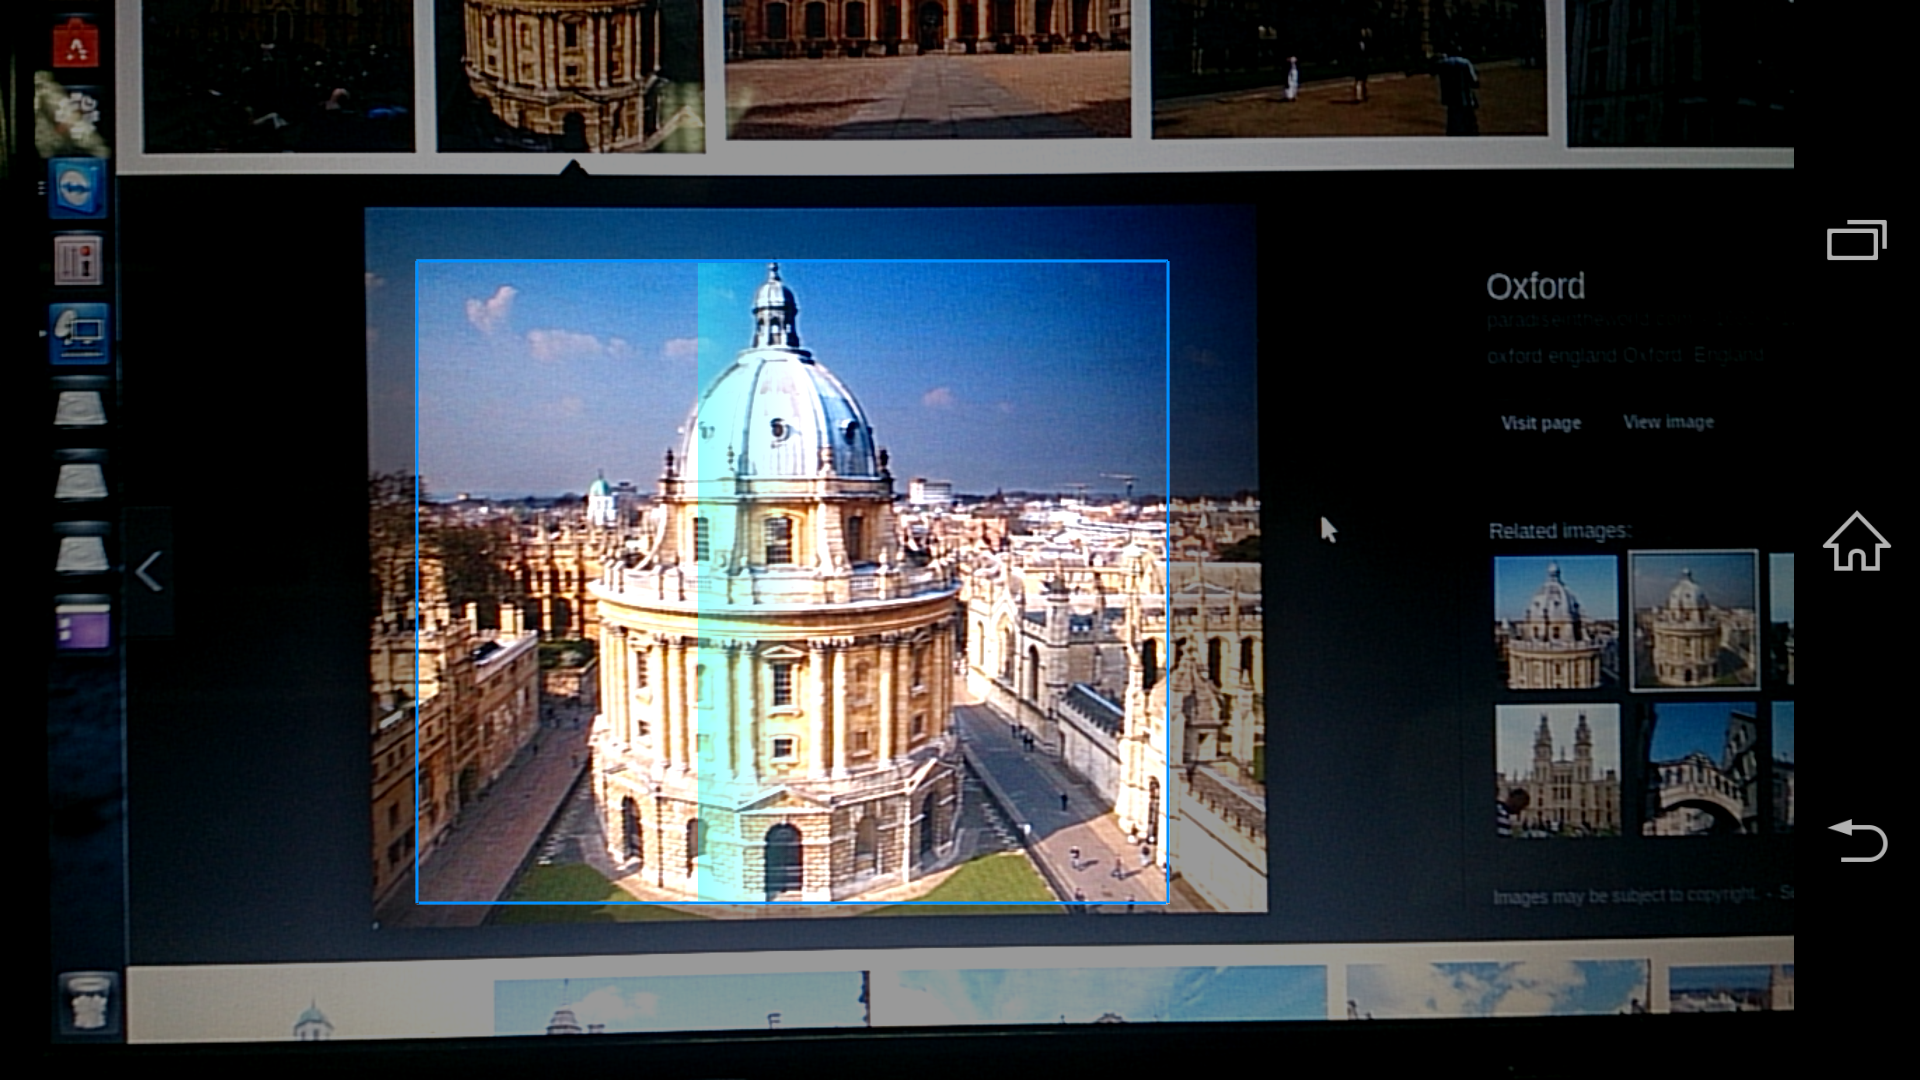
\includegraphics[scale=0.17]{processing}
    \fi
    \caption[Hình ảnh ứng dụng khi đang thực hiện truy vấn]{Hình ảnh ứng dụng khi đang thực hiện truy vấn.}
    \label{FigProcessing}
  \end{center}
\end{figure}

\begin{figure}[!htbp]
  \begin{center}
    \leavevmode
    \ifpdf
      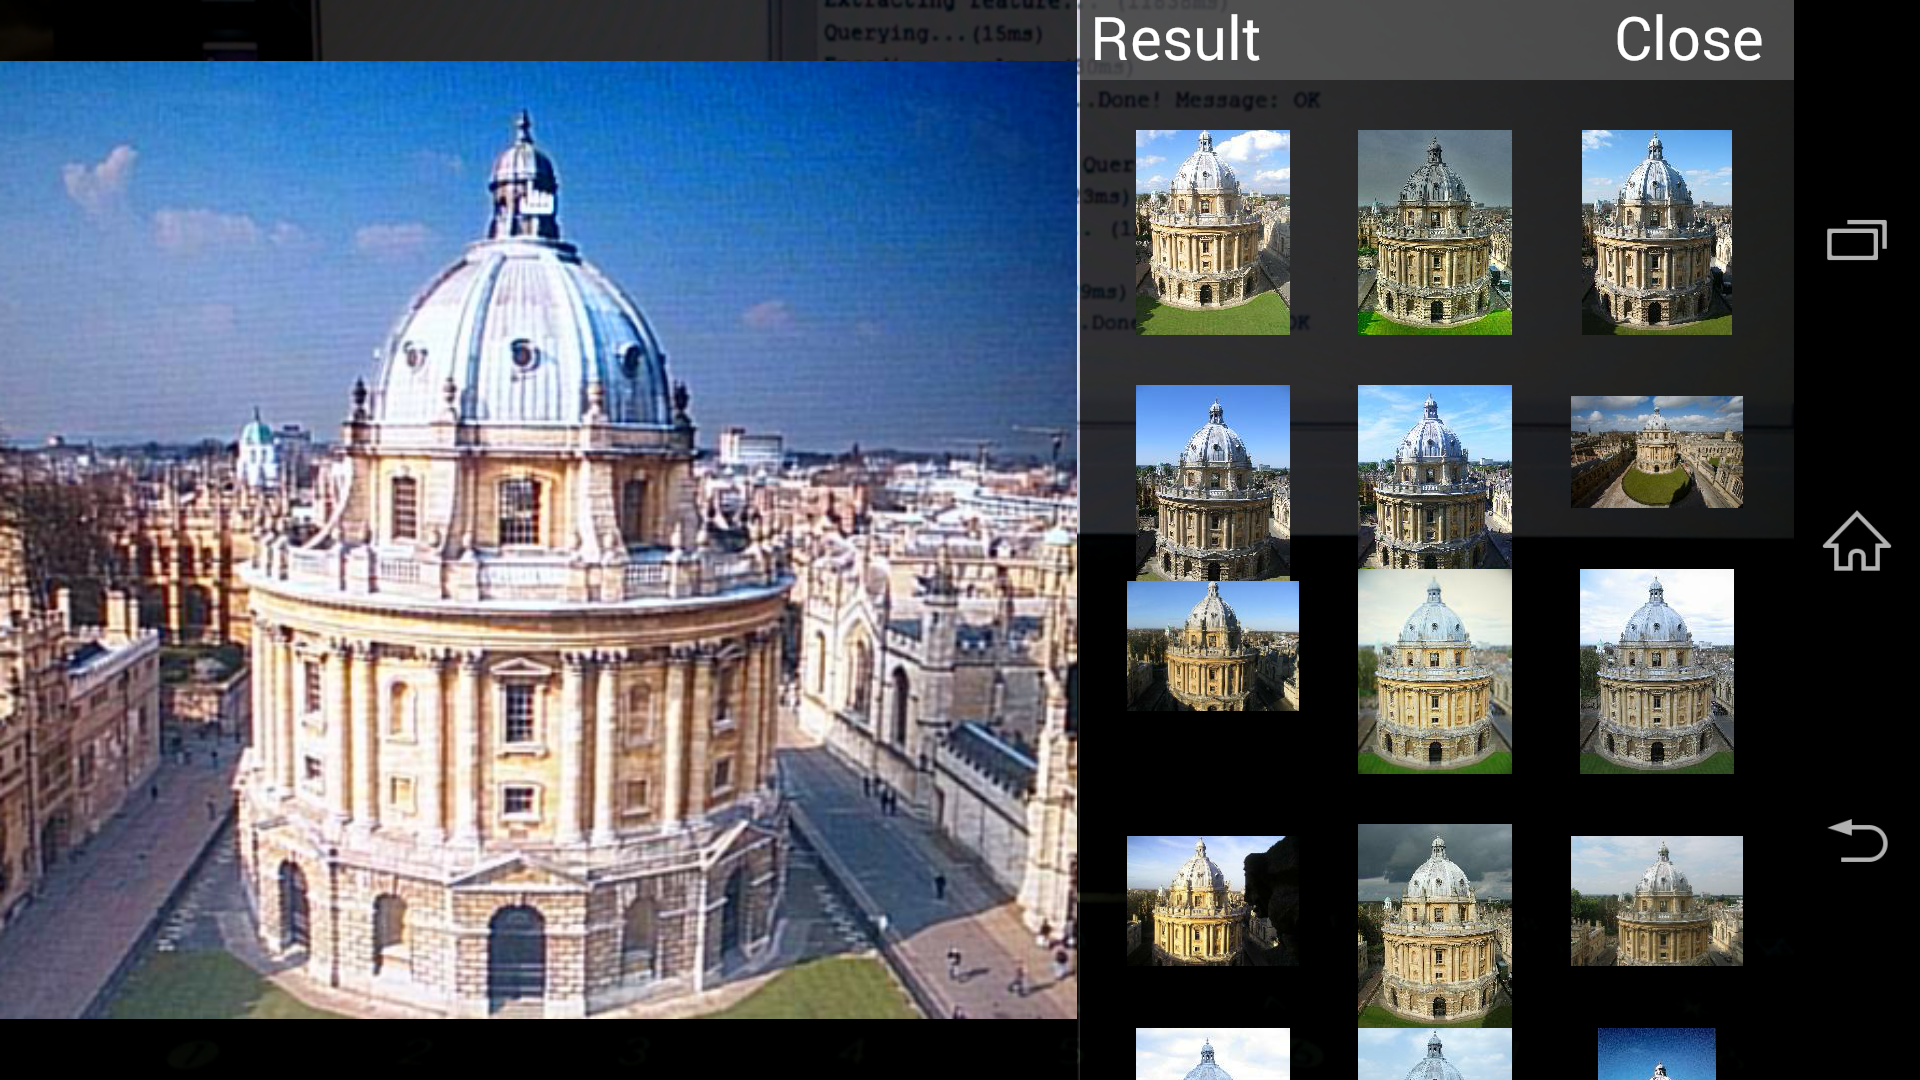
\includegraphics[scale=0.17]{result_capture}
    \else
      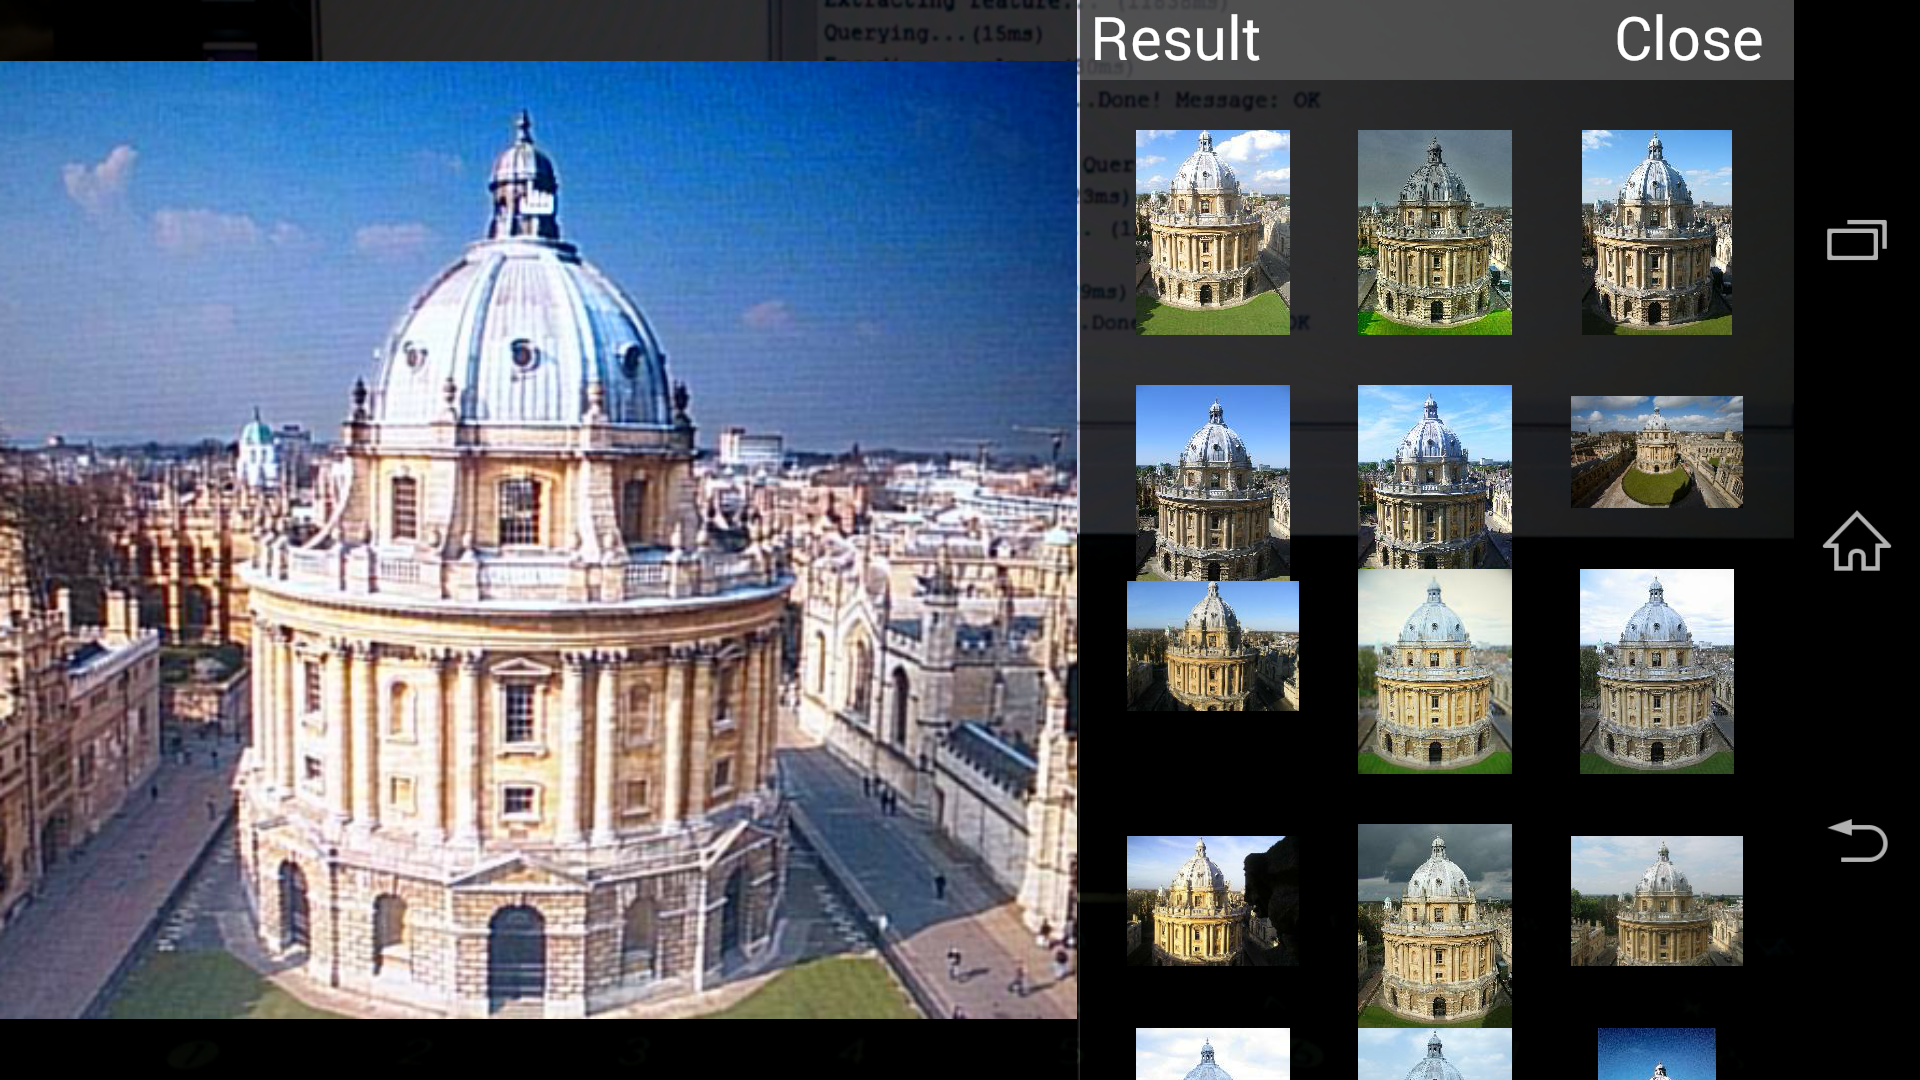
\includegraphics[scale=0.17]{result_capture}
    \fi
    \caption[Hình ảnh ứng dụng hiển thị kết quả truy vấn]{Hình ảnh ứng dụng hiển thị kết quả truy vấn.}
    \label{FigResultCapture}
  \end{center}
\end{figure}

\section{Cài đặt và thực nghiệm}
\label{c5-caidat}
	\subsection{Môi trường cài đặt}
	Môi trường cài đặt của hệ thống được liệt kê chi tiết dưới đây:
	
	\begin{itemize}
	\item \textbf{Processing Server:}
	
	-- Hệ điều hành: Windows Server 2008.
	
	-- Ngôn ngữ lập trình: Matlab, C.
	
	
	\item \textbf{Web Service:}
	
	-- Web server: Apache Tomcat 7.
	
	-- Ngôn ngữ lập trình: Java.
	
	
	\item \textbf{Client:}
	
	-- Hệ điều hành: Android.
	
	-- Ngôn ngữ lập trình: Java. 
	\end{itemize}	
	
	
	\subsection{Kết quả thực nghiệm}
	Ứng dụng nhóm xây dựng cho kết quả tốt. Ứng dụng chạy ổn định trên hệ điều hành Android. Thời gian trung bình cho mỗi truy vấn trên ứng dụng rơi vào khoảng 5 - 10s. Với những hình ảnh kích cỡ nhỏ thì thời gian truy vấn có thể chỉ trong 1s. Ngoài ra, thời gian truy vấn còn phụ thuộc vào nhiều yếu tố khác như điều kiện kết nối mạng hay chất lượng của hình ảnh truy vấn mà người dùng chọn.
	
	Ở đây, nhóm thực hiện thử nghiệm trên bộ dataset chuẩn đã dùng trong các thí nghiệm trước do đó độ chính xác không hề thay đổi so với kết quả của các thí nghiệm đã trình bày ở các chương trước.
	
	\subsection{Đánh giá kết quả}
	Kết quả thực nghiệm cho thấy ứng dụng tìm kiếm đối tượng trên ảnh đáp ứng được cơ bản các yêu cầu thực tế. Đồng thời, cách tổ chức hệ thống như trên cho phép người dùng hoàn toàn có thể scale ra nhiều server để đáp ứng được số lượng request lớn - một vấn đề mà các ứng dụng thực tế hiện nay phải đối mặt.
	
	Đồng thời, ứng dụng trên là nền tảng để phát triển vô số các ứng dụng thương mại khác vì ta có thể tùy biến trả về nhiều thông tin khác nhau tùy theo yêu cầu để ứng dụng cho nhiều lĩnh vực.